%% For double-blind review submission, w/o CCS and ACM Reference (max submission space)
% \documentclass[sigplan,twocolumn,review,anonymous]{acmart}
%\settopmatter{printfolios=true,printccs=false,printacmref=false}
\documentclass[letterpaper,twocolumn,10pt]{article}
\usepackage{usenix2019_v3}
% below add by chen
\usepackage[OT1]{fontenc}
% \usepackage{algorithm}
% \usepackage{algorithmicx}
% \usepackage[noend]{algpseudocode}
\usepackage{textcomp}
\usepackage{booktabs} % For formal tables\documentclass[conference]{IEEEtran}

% below add by chen
\usepackage[OT1]{fontenc}
% \usepackage{algorithm}
% \usepackage{algorithmicx}
% \usepackage[noend]{algpseudocode}
\usepackage{textcomp}
\usepackage{booktabs} % For formal tables
\usepackage{comment}
\usepackage{wrapfig}
\usepackage{xcolor}
\usepackage{graphicx}
\usepackage{subfig}
\usepackage{array}
\usepackage{multicol}
\usepackage{afterpage}
\usepackage{float}
\usepackage{listings}
\usepackage{multirow}
\usepackage{arydshln}
\usepackage{xspace}
\usepackage{enumitem}
\usepackage{fancyhdr}
\usepackage{amsmath}
\usepackage{url}
\usepackage[htt]{hyphenat}
\usepackage{subfloat}

\usepackage{amsfonts}
\usepackage{subcaption}
%\usepackage{subfigure}


\usepackage{cleveref}
\crefformat{chapter}{\S#2#1#3}
\crefformat{section}{\S#2#1#3} 
\crefformat{subsection}{\S#2#1#3}
\crefformat{subsubsection}{\S#2#1#3}

\graphicspath{{figures/}}

\usepackage{pifont}
\usepackage{xcolor}
\newcommand{\chen}[1]{\textcolor{red}{[#1]}}
\newcommand{\gz}[1]{\textcolor{blue}{[#1]}}
\newcommand{\yfliu}[1]{\textcolor{violet}{[#1]}}
\newcommand{\zhgan}[1]{\textcolor{teal}{[#1]}}
\newcommand{\ys}[1]{\textcolor{blue}{ys: [#1]}}
\newcommand{\phm}[1]{\vspace{.4em} \noindent\textbf{#1}\hspace{.5em}}

\usepackage{array}  
\renewcommand\arraystretch{1.3}
\usepackage{booktabs}
\usepackage{minted}

\usepackage{xcolor}
\usepackage[linesnumbered,ruled,vlined]{algorithm2e}
% \usepackage{amsmath}
% \usepackage{algorithmic}
% \usepackage{algorithmicx}
% \usepackage{algpseudocode}

%\acmConference[PL'18]{ACM SIGPLAN Conference on Programming Languages}{January 01--03, 2018}{New York, NY, USA}
%\acmYear{2018}
%\acmISBN{} % \acmISBN{978-x-xxxx-xxxx-x/YY/MM}
%\acmDOI{} % \acmDOI{10.1145/nnnnnnn.nnnnnnn}
%\startPage{1}


%% Copyright information
%% Supplied to authors (based on authors' rights management selection;
%% see authors.acm.org) by publisher for camera-ready submission;
%% use 'none' for review submission.
%\setcopyright{none}
%\setcopyright{acmcopyright}
%\setcopyright{acmlicensed}
%\setcopyright{rightsretained}
%\copyrightyear{2018}           %% If different from \acmYear

%% Bibliography style
%\bibliographystyle{ACM-Reference-Format}


\begin{document}

%% Title information
\title{Hermes: Towards Coinference-Centric Serving for LLM Applications} %Correlation-aware LLM Inference Serving}         %% [Short Title] is optional;
%\title{Hermes: Correlation-aware LLM Inference Serving}         %% [Short Title] is optional;
% \title{Hermes: CoInference-Centric Resource Scheduling for Modern LLM Workloads}
%\title{Hermes: Correlation-aware Request Scheduling for LLM Inference Workloads}         %% [Short Title] is optional;
                                        %% when present, will be used in
                                        %% header instead of Full Title.


%% Author information
%% Contents and number of authors suppressed with 'anonymous'.
%% Each author should be introduced by \author, followed by
%% \authornote (optional), \orcid (optional), \affiliation, and
%% \email.
%% An author may have multiple affiliations and/or emails; repeat the
%% appropriate command.
%% Many elements are not rendered, but should be provided for metadata
%% extraction tools.

%% Author with single affiliation.

\maketitle


\begin{abstract}
% Modern applications based on large language models (LLMs) are increasingly popular in recent years. 
% To accomplish a user task, such LLM-based applications usually issue a series of correlated LLM inference requests---with complex cross-request dependencies, dynamic per-request demand, and diverse inter-request tool calls.
% Existing LLM serving systems are oblivious to such correlations and suffer suboptimal performance when serving LLM applications. 

% In this paper, to leverage request correlations, we propose the \emph{coinference} abstraction to organize the correlated inferences.
% We then devise \emph{Hermes}, a coinference-centric LLM serving system.
% % also help to better capture inference-level resource demand, enabling a series of optimization techniques on intra-CoInference resource provisioning.
% Hermes first modeling coinference as a series of stages with detailed demand distributions.
% Second, leveraging the abstraction of coinference and its resource demands, Hermes implements a coinference-level scheduling algorithm, which is designed to ensure the multiple objectives of completing LLM applications efficiently.
% Third, with the resource demands, Hermes proposed a series of intra-coinference resource provisioning strategies to ensure the rapid completion of a LLM application.
% We have implemented Hermes atop vLLM with XX lines of code, and experimental results against diverse LLM applications show that Hermes can remarkably enhance the application-level service performance, e.g., reducing the average completion time by XX\%. 

Applications based on Large Language Models (LLMs) have become increasingly popular in recent years. 
To accomplish a high-level mission, LLM applications usually issue a series of correlated LLM inferences and non-LLM tasks, involving dynamic resource volumes, hybrid resource backends, as well as diverse performance objectives.
Existing LLM systems are oblivious to such characteristics, being suboptimal when serving LLM applications. 
In this paper, we abstract the resource demands of an LLM application into a \emph{coinference}, and further design \emph{Hermes}, a coinference-centric LLM serving system.
Hermes models a coinference as a list of functional stages---with built-in properties depicting inter-stage dependencies and intra-stage demands. 
Hermes further applies the Gittins policy to optimize inter-coinference scheduling performance against diverse objectives. % despite with demand dynamicity. 
Moreover, for fast serving of individual LLM applications, Hermes leverages the coinference-level demand model to coordinately provision the desired resources in various aspects like KV cache and non-LLM tools. 
We have implemented Hermes atop vLLM, and experiments with diverse LLM applications confirm that it can effectively improve the application serving efficiency, reducing the average completion time by up to 90\%. 

\end{abstract}




%% Keywords
%% comma separated list
% \keywords{keyword1, keyword2, keyword3}  %% \keywords are mandatory in final camera-ready submission


%% \maketitle
%% Note: \maketitle command must come after title commands, author
%% commands, abstract environment, Computing Classification System
%% environment and commands, and keywords command.

%!TEX root = main.tex
\section{Introduction}
\label{sec:intro}

% The recent years have witnessed the astonishing success of generative Large Language Models (LLMs)~\cite{brown2020language,floridi2020gpt,touvron2023llama} in revolutionizing various application domains~\cite{dosovitskiy2020image,stiennon2020learning,chen2021evaluating}.
% With ever widening adoption, LLM inference workloads are increasingly dominant in computing infrastructures of large companies or institutions.
% Serving an LLM inference request, which involves processing billion-scale model parameters for multiple generation iterations~\cite{yu_orca_2022},
% % is composed of a prefilling and a decoding phase, 
% usually demands plenty of memory and computing resources on GPUs~\cite{zhong_distserve_2024,agrawal_taming_2024}.
% For better user experience and lower operational cost, it is of paramount importance to serve the LLM workloads with fast response time and high resource utilization.

Large Language Models (LLMs)~\cite{brown2020language,floridi2020gpt,touvron2023llama} have been widely adopted in various domains~\cite{dosovitskiy2020image,stiennon2020learning,chen2021evaluating}.
Given the prohibitively high cost to train newer-generation LLMs, it is now more reachable to boost the power of LLMs by \emph{scaling-out} (i.e., building LLM-based applications) instead of by \emph{scaling-up} (i.e., adopting more advanced models)~\cite{compound_ai}. 
That is, by combining a set of LLM inference requests 
%in chain or parallel structure 
and also integrating with the non-LLM tools, users can improve the LLM performance in aspects like input length~\cite{jin2024comprehensive,lin2024infinite}, output reliability~\cite{chern2023factool,ji2023towards} and functional flexibility~\cite{shen2024hugginggpt,shen2024llm}.


% \chen{LLM applications issue multiple inference requests} 
% Specifically, with the emergence of various advanced LLM applications, there often exist obvious correlations among requests submitted to an LLM backend~\cite{lin2024parrot}.
% For example, prompt chaining frameworks like LangChain~\cite{topsakal2023creating} can statically code multiple LLM requests into an execution graph, with the output tokens of upstream requests working as the inputs of  downstream ones. 
% Meanwhile, chatbot verification applications like FacTool~\cite{chern2023factool} would launch multiple consecutive LLM inferences---respectively for question answering, claim extraction and search query generation---to accomplish a verification task.
% Besides, coding agents like MetaGPT~\cite{hong2023metagpt} may repeatedly issue similar LLM requests for an arbitrary number of times to ensure the coding quality in a self-reflection manner.  
% % Other applications like chain-style document summarization and 
% Note that, when running applications with such correlated requests, users primarily care about the \emph{end-to-end} performance---i.e., the time when all the constituting inferences complete---instead of the performance of individual inferences. \chen{add more explanations}

An LLM application refers to a group of LLM inferences, as well as the accompanying non-LLM tasks, that collaborate to accomplish a high-level mission for end users (\S\ref{sec:applications}).
		% For example, to ensure output reliabity, in Knowledge-based-Query-Answering application, each claims
%\chen{examples?}
%\yfliu{For example, to optimize traditional development workflows, the Code-Generation\cite{autogen} application can continuously generate code with the LLM and execute it with Docker, iteratively fixing errors and optimizing performance. }
Given the prevalence of such LLM applications, it becomes critical to serve them efficiently in clusters.
In particular, compared with traditional workloads, LLM applications have three distinct characteristics. 
First, the resource demand of LLM applications---like the text generation length and the total inference number---are dependent on the runtime inputs and uncertain a priori.
Second, serving LLM applications often requires coordinated provisioning of diverse resource backends (to support both LLM and non-LLM computations)~\cite{lewis2020retrieval,factool_code}. 
Third, LLM applications may have heterogeneous service objectives---some focus on end-to-end mission completion time~\cite{autogen,jin2024comprehensive}, yet some others care about instantaneous token generation speed~\cite{liu2024andes}.

% A series of research works have already been proposed in the literature to enhance the efficiency of serving LLM inference requests.
% For example, model quantization techniques~\cite{frantar2022gptq,kim2023squeezellm} can effectively mitigate per-iteration computation overhead; some other works like SpecInfer~\cite{miao2023specinfer} and Medusa~\cite{cai2024medusa} adopt speculative decoding to enhance token generation efficiency without compromising the output fidelity.
% Besides, \chen{change to attention-sparsification; add ORCA?} Zhong~et~al.~\cite{zhong_distserve_2024} and Agrawal~et~al.~\cite{agrawal_taming_2024} both proposed to separately host prefill and decoding computations on different GPUs to avoid prefill-decoding interference. \chen{examples can be compressed; main parts placed in Related Work section}
% However, the above works focus on accelerating individual LLM inferences yet ignore inter-request correlations, being suboptimal in end-to-end LLM serving performance. 
% \chen{add a toy example? describe the handover delay: wait for others in FIFO-based methods; even worse if with increasing parallelism}
% % However, all above works focus at the granularity of individual request---not aware of the correlations among different requests and thus suffering suboptimal performance. 
% % which we find, however, leaves a large uncharted torritory to further enhance the service effciiency of LLM workloads. 
% \ys{This paragraph is crucial as it presents this work's key problem / motivation. I suggest presenting concrete challenges as LLM-based apps move from simple chat to compound AI systems.
% The major issue is that the existing LLM serving systems only exploit inter-request dependency for KV cache reuse (various context caching works) but do not exploit scheduling optimizations.}

When serving LLM applications, existing works fail to work well in both inter-application scheduling and intra-application execution.
Most works in the literature focus on accelerating individual LLM inferences without awareness of the inter-request correlations~\cite{cai2024medusa,kim2023squeezellm,miao2023specinfer,frantar2022gptq,dao2022flashattention}, suffering suboptimal end-to-end performance due to inter-request delay. 
While some recent works can improve the performance of LLM applications~\cite{lin2024parrot,tan2024teola,liu2024andes,gao2024cost}, they focus on specific application types (e.g., chatbot) or optimization aspects (e.g., KV cache reuse), without dealing with the common characteristics of LLM applications.
Consequently, due to demand dynamicity, advanced scheduling algorithms like Shortest-Remaining-Processing-Time (SRPT) cannot be adopted when scheduling multiple LLM applications, nor can it be feasible to support diverse objectives. 
Meanwhile, without coordinated resource provisioning, an LLM application may be impeded on any resource backend due to contention or improper configuration. 



% In this paper, our goal is to improve LLM serving performance with awareness to request correlations.
% In particular, we abstract the correlated inferences into a \emph{CoInference}, and treat it as first-class citizen when scheduling LLM inference workloads. %when designing the LLM serving backend. 
% By leveraging \emph{built-in} (like with \emph{thread ID} in OpenAI Assistants APIs~\cite{assistants_api}) or \emph{customized} (like with \emph{Semantic Variables} designed by Lin~et~al.~\cite{lin2024parrot}) notations in LLM request message, it is easy for the LLM backend to identify---at runtime---the correlated inferences which constitute a CoInference. 
% Moreover, for a given LLM application, our empirical study show that
% % , albeit with diverse inputs, 
% its CoInference structure and resource demand is relatively stable across different trial runs, indicating strong predictability at the CoInference level.
% In general, the benefit of correlation-aware LLM serving is \emph{two-fold}. 
% % First, CoInference-centric serving can avoid potential inter-inference handover delay and grant fastpass to all the requests of a CoInference. %facilitate fast CoInference completion. %
% First, CoInference-centric serving can enable optimizing application-level scheduling objectives (e.g., minimizing the average \emph{application completion time}), which is the true concern of users.
% % avoid potential inter-inference handover delay and grant fastpass to all the requests of a CoInference. %facilitate fast CoInference completion. %
% Second, with CoInference-level modeling, the LLM service backend can capture the demand pattern of each request more precisely, and such information can facilitate proactive resource provisioning to speed up the completion of individual CoInferences. 
% \ys{The paper should clearly define what exactly is CoInfer, why it is called CoInfer (inspired by CoFlow), and list 1 or 2 examples to help readers understand. This is closely related to the use cases that are presented in earlier paragraphs.}

In this paper, we seek to enhance the scheduling and execution efficiency of LLM applications, and the key is to leverage request correlations.
To be specific, 
we propose an abstract called \emph{coinference}, 
%we abstract the correlated inferences of an application into a coinference, 
which organizes the correlated inferences of an LLM application in proper structure, and also records the non-LLM resource demands between LLM inferences.
% and treat it as the first-class citizen in LLM serving.
We note that with the built-in~\cite{assistants_api} or customized~\cite{OpenAI_extra_body} notations in LLM requests, it is easy for the LLM backend to identify the correlated inferences belonging to the same application.
The coinference abstraction can help to directly optimize 
%Coinference-centric serving can facilitate the optimization of 
the application-level scheduling objectives.
Moreover, for a given LLM application, our empirical study shows that its resource demand is relatively stable across different trial runs with diverse inputs; therefore, with coinference-level demand modeling, we can more precisely predict the demand information of the entire application as well as of each request, which can further facilitate application scheduling and resource provisioning. 


Based on the coinference abstraction, we design \emph{Hermes}, a coinference-centric serving system for LLM applications, with the objective of achieving improved efficiency in both inter-application scheduling and intra-application execution.
In our Hermes design, we address the challenging characteristics of LLM applications (i.e., demand dynamicity, objective diversity, and resource hybridity) with three modules: coinference demand modeling, inter-coinference scheduling, and intra-coinference resource provisioning. 

% Based on the CoInference abstraction, we further design Hermes, a CoInference-centric LLM serving system that can improve LLM application performance and resource utilization.
% Our Hermes design is composed of three main parts: CoInference demand modeling, inter-CoInference scheduling, and intra-CoInference resource provisioning. 
% \ys{It's unclear to me what is Hermes, what are challenges building it, and how it works in general. My understanding is that Hermes has two parts, an offline profiler and an online runtime. The offline profiler profiles a given LLM-based applications and outputs a set of specs. During runtime, the Hermes online runtime will take the output and schedule requests from this app accordingly. The Hermes online runtime is likely a self-contained LLM serving system with a global scheduler and multiple vLLM instances. It is also crucial to highlight how each proposed technique overcome new challenges enabled by compound LLM-based apps.}

% First, we design a general multi-stage paradigm to model the CoInference resource demands for general LLM applications, laying the foundation for CoInference-level optimizations. 
% In that paradigm, each stage corresponds to a functioning phase of the LLM application (e.g., for claim extraction in FacTool~\cite{chern2023factool}), which contains one or multiple parallel inference requests. 
% Within a stage, we profile an extensible set of demand aspects---like the number of LLM requests or \emph{stage parallelism}, output token length, kv-cache size, time gap to the downstream stage (all necessary for our later optimizations). 
% Moreover, despite application-specific demand similarity, we note that a CoInference's runtime resource demand may still exhibit salient uncertainty in multiple levels---even the number of stages in a CoInference may be dynamic;
% to handle such uncertainty, we add special primitives to indicate looping stages, and adopt Normal distribution to describe such fluctuating demand quantity. 
% To summarize, with CoInference awareness, we can make more precise demand modeling for LLM inference requests in a structured and probabilistic manner. 

First, we devise a general and precise method for coinference demand modeling.
			%To describe the diverse request relationships, we model a coinference as a list of stages, w
For generality, we model a coinference as a list of \emph{stages}, where each stage represents a functional unit with one or multiple parallel requests.
In each stage, we record a series of properties to express request dependencies, looping status and even non-LLM demands. %\yfliu{Is this sentence necessary?}
For preciseness, we choose to record the resource demands in each aspect (e.g., input/output token length, request parallelism) as a distribution rather than a single constant, trying to preserve the panoramic demand information; we also notice the demand correlations between dependent requests and further adopt correlation analysis to enhance the demand prediction accuracy at runtime. 

% \chen{To be largely rewritten}
% Second, in resource contention, we seek to emulate Shortest-CoInference-First with the conventional inference-level scheduling primitives.
% Specifically, Hermes assign different scheduling priorities to the pending CoInferences based on their overall service cost previously profiled; each inference---which is the actual scheduling unit in existing LLM serving frameworks like vLLM~\cite{vllm}---inherits the priority from the CoInference it belongs to. 
% This way, we can ensure that all the constituting requests of a small (high-priority) CoInference can be executed smoothly without being backlogged. 
% We also introduce special designs for the cases where a request's CoInference affiliation is absent or the profiled CoInference serving cost turns out inaccurate at execution time.  \chen{shortest remaining job first with the context switching overhead considered?}

Second, we design a scheduling algorithm that can minimize the average completion time of LLM applications, and further extend it to support diverse objectives. 
%Our previous coinference modeling cannot eliminate the resource dynamicity, 
Confronting uncertain demands with distribution-like description, the classical SRPT algorithm is no longer optimal. 
For scheduling LLM applications, Hermes instead applies Gittins policy~\cite{aalto2009gittins, scully2021gittins}, which has been proven optimal for jobs with unknown demand but known demand distributions. 
Moreover, when concurrently serving applications with SLO objectives (e.g., on deadline or instantaneous generation speed), Hermes keeps identifying and prioritizing the ones with a high risk of SLO violation, and the remaining applications are scheduled under the default SRPT-like policy.

% \chen{To be rewritten} Third, to efficiently serve individual CoInferences, Hermes is equipped with speculative resource provisioning.
% % LLM inference serving is resource-intensive in both computation and memory; 
% Under intense resource contention, reactive resource provisioning (i.e., acting only after LLM requests arrive) would yield non-negligible startup delay.
% For example, to provision enough memory space for the incoming high-priority requests, the LLM engine may have to evict some running inferences with their KV-cache swapped out, which is time consuming~\cite{wu2023fast}.
% That problem would be even more severe when the request parallelism drastically increases in downstream stages (common in applications like FacTool~\cite{chern2023factool}).
% In Hermes, we leverage the CoInference modeling to estimate the arrival time and parallelism of downstream stages, thereby realizing proactive resource provisioning. 
% % Meanwhile, after a CoInference stage completes, the LLM engine often witnesses nongliegible time gap prior to the request arrival of the downstream stage---due to factors like round-trip time or non-LLM computations in-between.
% In addition, frequently interrupting the execution of low priority inferences would cause large KV-cache swapping overhead; to attain high resource utilization, after a high-priority inference finishes, Hermes preferentially executes the low-priority inferences that are likely to complete before the arrival of downstream high-priority requests.
			
%Third, for intra-application resource provisioning, we apply the demand information from coinference modeling for the management of the diverse resource backends.
Third, for the efficient execution of individual applications, we propose coinference-aware clairvoyant resource provisioning, applying the demand information from coinference modeling for management of the diverse resource backends.
%  (all could be the service bottlenecks for LLM applications).
%When managing the GPU memory storing KV cache~\cite{kwon2023efficient} and LoRA adaptors~\cite{hu2021lora}, we propose to determine the cache eviction order based on the coinference priority and the cache prefetching moments based on the profiled distribution of inter-stage gaps. 
When managing the storage space of KV cache~\cite{kwon2023efficient} and LoRA adaptors~\cite{hu2021lora}, we propose clairvoyant cache management to determine the cache eviction order based on the coinference priority and the prefetching moments based on the profiled distribution of inter-stage gaps. 
When managing non-LLM backends like CPU (to launch docker container) and network (to conduct RAG), we propose clairvoyant queueing that propagates the coninference priority to each resource backend.
In cases with multiple LLM backends with heterogeneous batch size configurations, we propose clairvoyant backend selection, which means adaptively selecting the backend for each stage based on the profiled request parallelism. 
These methods can ensure that an LLM application can have fast completion without being impeded on any resource backends.

We have implemented Hermes with over 4,100 lines of Python code atop vLLM, a popular LLM serving framework.
%We replace the default vLLM scheduler to \texttt{CoinferenceScheduler}, which leverages the demand information from the \texttt{CoInferenceAnnotator} for scheduling and also propagates the resource provisioning hints to lower-level resource managers. 
%\yfliu{I'm not sure. Do we need to show the implementation details in introduction? }
We evaluate Hermes performance against mainstream schedulers with a diverse set of modern LLM applications. 
Experimental results show that Hermes can improve the average application completion time by up to 90.1\% while providing a near-optimal SLO guarantee. 
Ablation studies also confirm the effectiveness of our approaches in tacking demand dynamicity as well as in efficient resource provisioning on diverse backends. %for individual coinferences.   

% We have implemented Hermes with two components: a Coinference-aware request annotator and a Coinference-aware LLM service engine.
% The request annotator maintains a profiled knowledge base which depicts the Coinference structure and demand pattern for each application.
% Based on the Coinference modeling knowledge, the annotator diagnoses the stage affiliation of each incoming request, and associates it with the auxiliary annotations (e.g., scheduling priority, kv-cache consumption). 
% \chen{add stage-handler? trigger and supervise the execution of a stage? or annotator is a stage-brain? two modules or three modules?}
% The Coinference-aware LLM service engine is customized to understand such annotations; 
% %it will schedule the request and 
% it will make request scheduling and resource provisioning decisions accordingly after annotated requests arrive. % each request.
% %the LLM service engine makes request scheduling and resource provisioning decisions according to the auxiliary annotation. 
 
% To evaluate the performance of Hermes, we build a benchmark workload suite containing XXX. 
% In end-to-end evaluation, Hermes can reduce the average Coinference completion time by XX\%.
% Moreover, even when the Coinference knowledge is inaccurate or absent, Hermes can still attain a performance enhancement of XX\%.
% Extensibility and future work...  

% \ys{Please also list this paper's main contributions.}
%!TEX root = main.tex
\section{Background and Motivation}
\label{sec:background}

\subsection{LLM Applications: A Primer}
\label{sec:applications}

\subsubsection{The trend towards LLM applications.} 
Large language models (LLMs)~\cite{brown2020language,floridi2020gpt,touvron2023llama} stand out as a general technique whose intelligence capability can potentially be applied to various domains~\cite{dosovitskiy2020image,hadi2023survey}. 
Yet, even though AI models are evolving rapidly~\cite{sonoda2024diagnostic,reid2024gemini}, it is commonly recognized that a single LLM request is often deficient when addressing realistic problems. 
For example, the input context windows of typical LLMs are often of limited sizes (less than 10M tokens)~\cite{chen2023extending,lin2024infinite}, thus processing a large document would require issuing multiple parallel inference requests. 
Meanwhile, LLMs are plagued by the problem of \emph{hallucination}~\cite{ji2023survey}, meaning that the output of a single LLM request may be unfaithful or nonsensical, and some additional LLM requests are then required to ensure LLM output quality (for example, with FacTool~\cite{chern2023factool} verifications or with self-reflection~\cite{ji2023towards}).
Besides, the built-in knowledge and capability of LLMs are usually insufficient in professional occasions, thus various non-LLM components (e.g., knowledge retrieval~\cite{lewis2020retrieval}, third-party tools~\cite{shen2024llm} or other small models~\cite{shen2024hugginggpt}) are commonly adopted to augment LLM capabilities~\cite{abhyankarinfercept}, as 
%such functionalities are commonly 
integrated in LLM agents like AutoGPT~\cite{fezari2023gpt} and MetaGPT~\cite{hong2023metagpt}. 
To summarize, to enlarge the input length, improve the output reliability, and integrate more functionalities, LLM practitioners often need to conduct multiple inferences with the necessary non-LLM computations, which form a compound workflow.
% \ys{What exactly are LLM applications? Is LLM-based chat an LLM app? Yes, it is. I think the main trend is that to mitigate LLM hallucination and to improve AI accuracy at complex reasoning tasks, LLM-based apps have evolved from single-turn LLM-based chat to a more compound and complicated workflow. Then list examples such as RAG, o1, factool etc.}

We call the above compound workflow---with multiple LLM requests and even non-LLM tasks to accomplish a realistic mission---as an \emph{LLM application}.
LLM applications are rapidly emerging in recent years~\cite{hadi2023survey,tan2024teola,lin2024parrot}, and have become an increasingly prevalent workload type in production clusters.
Fig.~\ref{fig:app_structure} presents the structures and descriptions of ten typical LLM applications\footnote{
We deem multi-turn conversation as a special application whose mission is to help users obtain the desired information via iterative LLM interaction.
Moreover, in solution design, we do not particularly differentiate AI agents~\cite{fezari2023gpt,hong2023metagpt} from other applications, because the definition of agent itself is vague, and the typical components of AI agents, like ReActing, planning, RAG, and tool-calling, have all been considered in our modeling of LLM applications.
Finally, we admit that it is impossible to exhaustively list all the LLM applications here, but we believe the applications in Fig.~\ref{fig:app_structure} are sufficiently representative because they cover the essential characteristics of general LLM applications (as summarized later in Table 1). 
}
studied in this paper.


\begin{figure*}
    \centering
    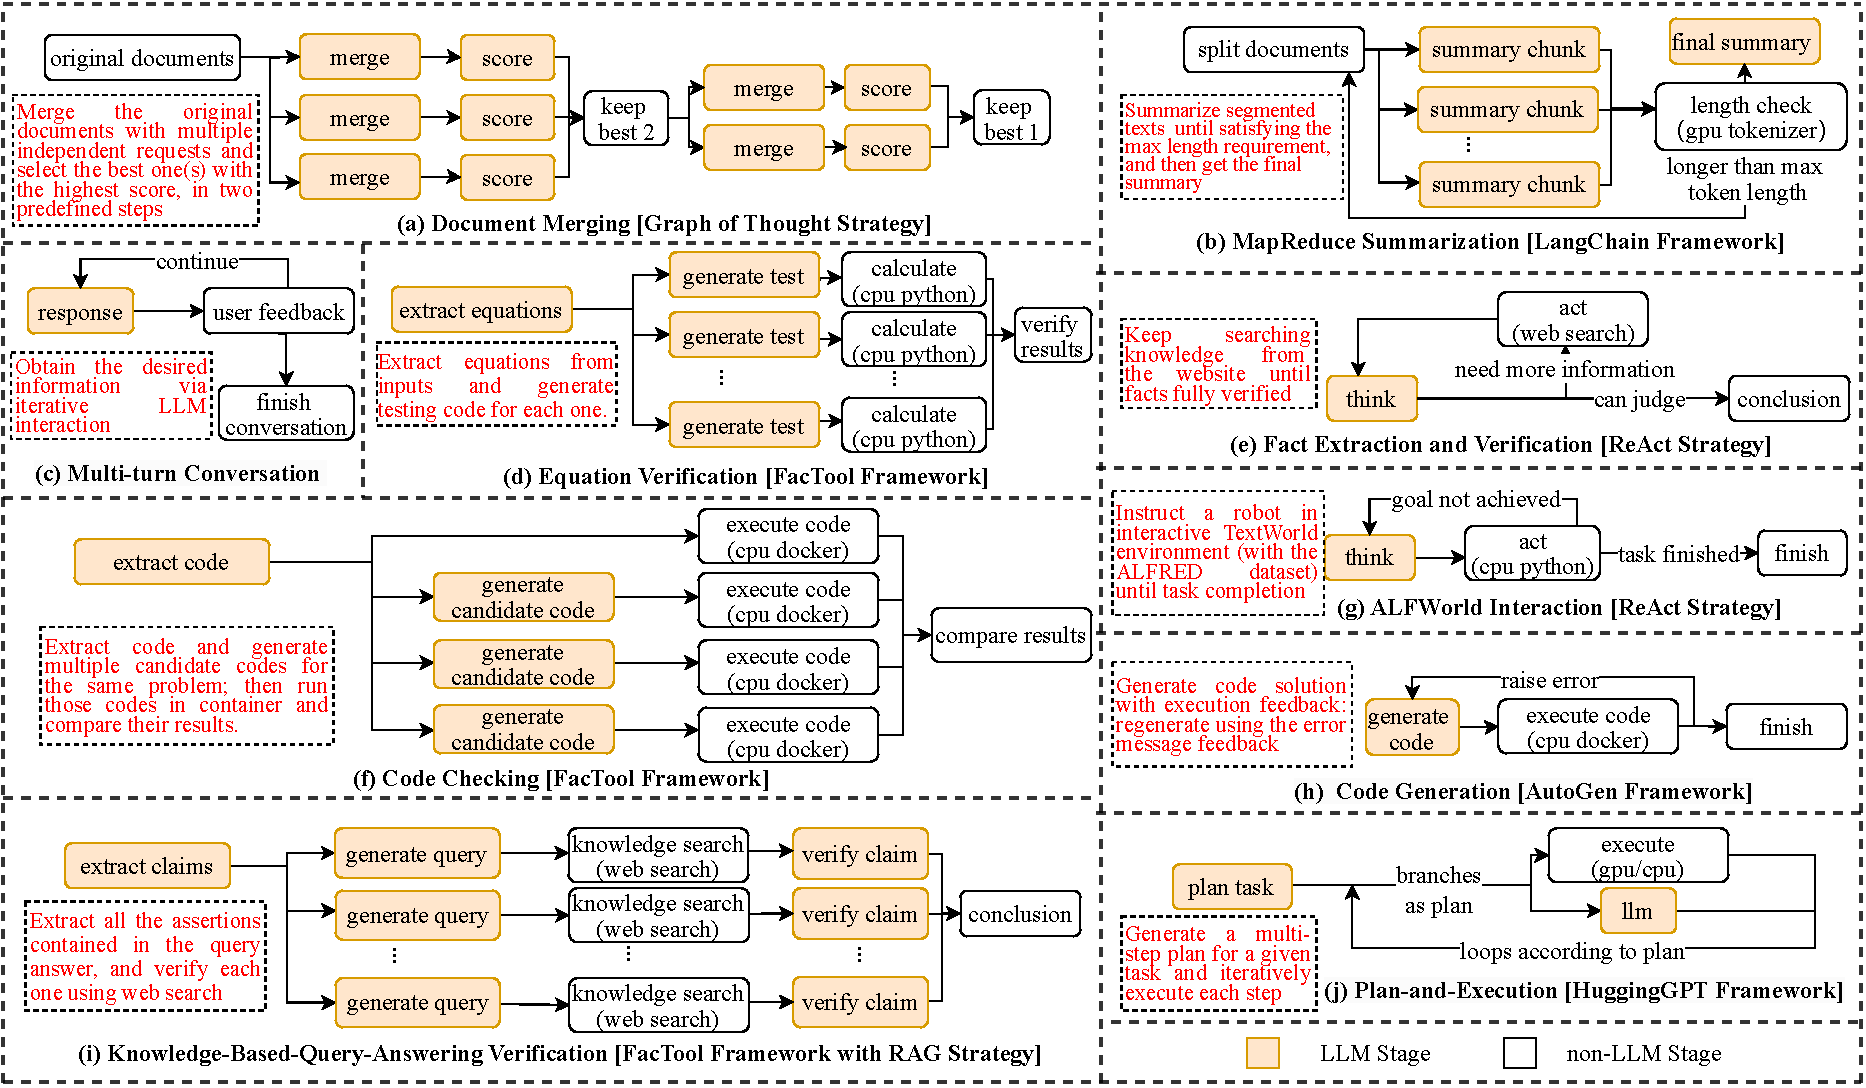
\includegraphics[width=0.96\textwidth]{figures/app structure.pdf}
    \caption{The structures of typical LLM applications (sources listed in Table 1). An application can be built with dedicated frameworks (e.g., FacTool and AutoGen) or following certain control strategies (e.g., Graph of Thought and ReAct). }
    %Used Applications. \chen{add brief introduction and source citation} \chen{add conversation and planning?} \chen{place description directly in figures? Summary the common patterns in title instead?} \gz{multi-turn conversation fault}}
    \label{fig:app_structure}
    \vspace{-0.1in}
\end{figure*}

%\ys{For the following characteristics, we could add another subsection with the name like "Challenges of Compound LLM Applications". In all, this subsection is used to present challenges, aka motivation, problem statement of this paper.}
\subsubsection{Challenging characteristics of LLM applications.}
The serving quality of LLM applications is critical to user experience and the total service profit. 
Nonetheless, it is indeed quite challenging to efficiently serve the LLM applications given their distinct characteristics as follows:

 \emph{1) Demand Dynamicity.}
        The resource demand of LLM applications exhibits strong dynamicity on two levels. %both inter-request level and intra-request level.
        First, the application structure (i.e., the number and organization of the constituting requests) may be uncertain in advance.
        Although some applications (like the hard-coded inference workflows with LangChain~\cite{topsakal2023creating}) have a fixed structure, for some other applications with ReActing~\cite{ji2023towards,yao2022react} or LLM-planning~\cite{shen2024hugginggpt}, the application structure can only be determined at runtime based on the inference contents. 
        Second, for each individual request, as pointed out by many existing works~\cite{gao2024cost,wu2023fast}, both the input and output token lengths are dynamic.
        This implies that the inference duration and peak memory consumption (which are positively correlated with the number of tokens) are also difficult to predict a priori.
        
 \emph{2) Resource Hybridity.}
        While LLM inferences with GPU backends are the mainstream computations in LLM applications, there also exist various non-LLM tasks in many agent-like applications. 
	Those non-LLM tasks demand additional resources other than GPUs.
	For example, in the code-generation application provided by the FacTool framework, the LLM-generated codes need to be tested on CPU backends (e.g., with a        docker container~\cite{factool_code}). 
	Meanwhile, remote knowledge retrieval~\cite{lewis2020retrieval} would consume network resources. 
        Efficient serving of LLM applications would require coordinated provisioning of such hybrid resources. % need to be coordinated well for efficiently serve the LLM applications. 
        
 \emph{3) Objective Diversity.}
        Different LLM applications, based on their respective service contents, may have different performance objectives.
        For example, for many applications where only the final outputs matter---like document-summarization~\cite{jin2024comprehensive} or code-generation~\cite{autogen}, users only care about the ultimate application completion time.
        Meanwhile, applications may also have different service level objectives: for applications whose intermediate results need to be timely returned to users---like conversational text streaming services~\cite{liu2024andes}, the performance objective is to attain high instantaneous generation speed (as measured by the \emph{Time-To-First-Token} and \emph{Time-Per-Output-Token} metrics~\cite{zhong_distserve_2024}).
        In some other cases, the performance objective can also be to get the final output prior to the specified deadline~\cite{nie2024aladdin}. 
        We note that the performance objective is a built-in property of an LLM application, which shall be indiscriminately respected in scheduling.
        
In Table 1, we check each application in Fig.~\ref{fig:app_structure} against the above aspects, which suggests that those characteristics are quite common for modern LLM applications.
Note that such characteristics are significantly different from the traditional model serving workloads prior to the LLM era~\cite{crankshaw2017clipper,zhang2019mark} (which have fixed inference time, only consume GPU resources, and share the same performance objective).
In a nutshell, to design an ideal serving system for LLM applications, we need to properly deal with such distinct characteristics, seeking to yield high service quality at the application level---which is directly perceived by end users.
%ideal LLM serving system shall
%Confronting the above challenges, an ideal LLM serving system shall
%behave well in application-level service quality to guarantee the ultimate user experience.
%be able to yield high service quality at the application level for good user-perceptive experience.
%\ys{do we have experiments that can be used to motivate work? If so, we can put some here.}

\begin{table}
\centering
\resizebox{\linewidth}{!}{
\begin{tabular}{|c|c|c|c|c|c|c|c|c|}
\hline
\multirow{2}{*}{Task} & \multicolumn{3}{|c|}{Demand Dynamicity} & \multicolumn{2}{|c|}{Resource Hybridity} & \multicolumn{3}{|c|}{Objective Diversity}\\  \cline{2-9}
                                   & Structure & Parallelism & I/O              & GPU       & Non-LLM backends                      & ACT       & DDL       & TPT \\ \hline
(a) DM \cite{got_docmerge}        & \ding{55} & \ding{55}   & \ding{51}       & \ding{51} & \ding{55}       & \ding{51} & \ding{51} & \ding{55}  \\ \hline
(b) MRS \cite{Langchain_MapReduce} & \ding{51} & \ding{51}   & \ding{51}       & \ding{51} & \ding{51} (GPU: tokenizer)      & \ding{51} & \ding{51} & \ding{55}  \\ \hline
(c) MC \cite{sharegpt}            & \ding{51} & \ding{55}   & \ding{51}       & \ding{51} & \ding{55}       & \ding{55} & \ding{55} & \ding{51}  \\ \hline
(d) EV \cite{factool_math}        & \ding{55} & \ding{51}   & \ding{51}       & \ding{51} & \ding{55}      & \ding{51} & \ding{51} & \ding{55}  \\ \hline
(e) FEV \cite{react_fever}         & \ding{51} & \ding{55}   & \ding{51}       & \ding{51} & \ding{51} (Network: search)      & \ding{51} & \ding{51} & \ding{55}  \\ \hline
(f) CC \cite{factool_code}        & \ding{55} & \ding{55}   & \ding{51}       & \ding{51} & \ding{51} (CPU: docker)       & \ding{51} & \ding{51} & \ding{55}  \\ \hline
(g) ALFWI \cite{react_alfw}          & \ding{51} & \ding{55}   & \ding{51}       & \ding{51} & \ding{55}    & \ding{51} & \ding{51} & \ding{55}  \\ \hline
(h) CG \cite{autogen}             & \ding{51} & \ding{55}   & \ding{51}       & \ding{51} & \ding{51} (CPU: docker)       & \ding{51} & \ding{51} & \ding{55}  \\ \hline
(i) KBQAV \cite{factool_kbqa}        & \ding{55} & \ding{51}   & \ding{51}       & \ding{51}  & \ding{51} (Network: search)   & \ding{51} & \ding{51} & \ding{55}  \\ \hline
(j) PE \cite{hugginggpt}          & \ding{51} & \ding{55}   & \ding{51}       & \ding{51} & \ding{51} (GPU: small models)      & \ding{51} & \ding{51} & \ding{55}  \\ \hline
\end{tabular}
}

\vspace{0.1in}
\caption{
Characteristics in aspects of \emph{demand dynamicity}, \emph{resource hybridity} and \emph{objective diversity} for the LLM applications in Fig.~\ref{fig:app_structure} (for conciseness, hereafter we use the uppercase letter abbreviation to represent each application).
Regarding the objectives, ACT means to reduce Application Completion Time, DDL means to meet a preset completion deadline, and TPT means to guarantee the instantaneous performance on \emph{time per (processed) token} (for simplicity, here we do not differentiate prompt or completion tokens).
%The classification of applications. As seen in the table, our workloads cover all three different types of Demand Dynamicity and require backends using different resources. Moreover above applications have three different performance or service level objectives. So we could claim that our testbed is sound and diversity.(for conciseness, we use the uppercase letter abbreviation to represent each application), 
}
\vspace{-0.1in}
\end{table}

\subsection{Prior Arts and Their Limitations}

% \begin{figure}
%     \centering
%     \includegraphics[width=0.5\linewidth]{example-image-a}
%     \caption{request scheduling vs. good CoInference scheduling vs. bad CoInference scheduling}
%     \label{fig:toy_example}
% \end{figure}

% \ys{This is the background and motivation section not the Related Work section hence we should keep this simple so readers do not get lost. My suggestion is emphasize on works that deal with agent scheduling, inter-request scheduling etc. This is a relatively new field. I think only these papers qualify: Parrot and Teola. Experts will ask (a) what is the design space of agent/multiple-LLM scheduling; (b) WHY parrot and Teola cannot solve the challenges presented above; (c) finally, what's new with CoInfer and Hermes, what's our key insight.}

% In the literature, a bewildering array of research works have appeared on improving LLM inference performance.
% In \emph{operator implementation} aspect, the FlashAttention~\cite{dao2022flashattention} and FlashDecoding~\cite{hong2024flashdecoding} style algorithms are commonly adopted to realize efficient LLM inference by integrating IO awareness. 
% In \emph{model deployment} aspect, model-quantization~\cite{frantar2022gptq,kim2023squeezellm}, paged-attention~\cite{kwon2023efficient} and prefill-decode-separation~\cite{zhong_distserve_2024,agrawal_taming_2024} methods have been proposed to maximize backend utilization.
% In \emph{inference algorithm} aspect, continuous batching~\cite{yu_orca_2022} and speculative decoding methods~\cite{miao2023specinfer,cai2024medusa} are also applied to improve the inference throughput.
% In \emph{request scheduling} aspect, a series of request-level scheduling algorithms like FastServe~\cite{wu2023fast} and Llumnix~\cite{sun2024llumnix} have emerged to improve the overall serving performance. 
% Yet, those inference-level optimizations are oblivious to the correlation of the requests belonging to the same LLM application, often being sub-optimal in application-level performance. 

In the literature, many research works have been proposed on optimizing LLM inferences in aspects like operator implementation~\cite{dao2022flashattention,hong2024flashdecoding}, model deployment~\cite{frantar2022gptq,kim2023squeezellm,kwon2023efficient,zhong_distserve_2024,agrawal_taming_2024} and inference algorithm~\cite{yu_orca_2022,miao2023specinfer,cai2024medusa,wu2023fast,sun2024llumnix}.
%~\cite{dao2022flashattention,kim2023squeezellm,miao2023specinfer,sun2024llumnix,cai2024medusa}.
Nonetheless, they mostly focus on individual inference requests, being oblivious to the request correlations and often suffering sub-optimal application-level performance. 
In particular, when scheduling multiple requests, the default policy adopted in popular inference frameworks like vLLM~\cite{vllm} is First-Come-First-Serve (FCFS) (largely due to demand uncertainty). 
Fig.~\ref{fig:toy_example} shows two LLM applications (A and B) served by a LLM engine (which we assume can serve only one request at a time, i.e., with a batch size of 1).
The default request-level FCFS scheduler (Fig.~\ref{subfig:request-level fcfs}) would interleave the inference serving of different applications, leading to long average Application Completion Time (ACT).
However, if we prioritize all the inference requests of B over A (Fig.~\ref{subfig:prioritize B over A}), we can substantially reduce the average ACT. 
%\chen{So for the objectives on instantaneous time-per-output-token}
% \ys{probably should move this toy example and its test numbers to the Problem Statement part.}

\begin{figure}
    \vspace{-.18in}
    \centering
    \subfloat[\vspace{-0.1in}Request-level FCFS]
    {
        \label{subfig:request-level fcfs}
        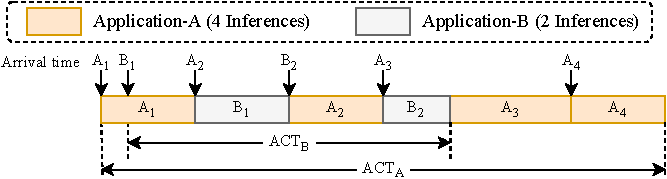
\includegraphics[width=6cm]{figures/scheduling_motivation/request_level_fcfs.drawio.pdf}
    }\hfill
    \subfloat[\vspace{-0.1in}Prioritize B over A]
    {
        \label{subfig:prioritize B over A}
        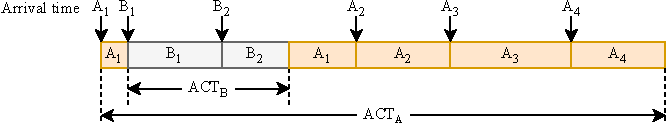
\includegraphics[width=6cm]{figures/scheduling_motivation/prioritize_b_over_a.drawio.pdf}
    }\hfill
    \subfloat[\vspace{-0.1in}Prioritize A over B]
    {
        \label{subfig:prioritize A over B}
        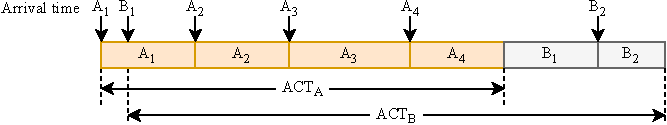
\includegraphics[width=6cm]{figures/scheduling_motivation/prioritize_a_over_b.drawio.pdf}
    }\hfill
    \caption{A toy example showing the scheduling algorithms' impact on the overall performance of two LLM applications (A and B, respectively with 4 and 2 dependent LLM requests indexed by the subscripts).
    Compared with request serving in FCFS (first-come-first-serve) manner, prioritizing all requests of B over A can yield a shorter average ACT (Application Completion time), yet an improper order (prioritizing A over B as in FCFS manner) leads to a worse performance.}
    \label{fig:toy_example}
\end{figure}

Apart from accelerating individual LLM inferences, there do exist some recent works on improving the performance of LLM applications.
For example, Parrot~\cite{lin2024parrot} employs a simple heuristic that schedules the requests of an application together to optimize the end-to-end performance. 
%proposes to identify the correlated inferences with the notion of semantic variables, and 
However, merely executing the correlated request together is not enough: as shown in Fig.~\ref{fig:toy_example}, the average ACT when instead prioritizing A over B (Fig.~\ref{subfig:prioritize A over B}) is even worse than the default case (Fig.~\ref{subfig:request-level fcfs}). 
%There are some other methods on application level optimizations: 
Apart from Parrot, CachedAttention~\cite{gao2024cost} and Infercept~\cite{abhyankarinfercept} focus on improving the effectiveness of KV-cache reusing between dependent requests of an LLM application; 
Teola~\cite{tan2024teola} applies compilation and batching optimizations to accelerate individual applications; 
Andes~\cite{liu2024andes} seeks to improve the instantaneous token generation performance for text streaming services. 

\begin{figure*}
            \vspace{-.1in}
	\parbox[t]{18cm}{
		\centering
		{
			\centering
			
\includegraphics[width=3.2cm]{figures/prompt/0.pdf}
			\label{fig:p_token_factoolcode}
		}\hfill
		{	
			\centering
			
\includegraphics[width=3.2cm]{figures/prompt/3.pdf}
			\label{fig:p_token_gotdecmerge}
		}\hfill
		{	
			\centering
			
\includegraphics[width=3.2cm]{figures/prompt/1.pdf}
			\label{fig:p_token_factoolkbqa}
		}\hfill
		{	
			\centering
			
\includegraphics[width=3.2cm]{figures/prompt/2.pdf}
			\label{fig:p_token_factoolmath}
		}\hfill
		{	
			\centering
			
\includegraphics[width=3.2cm]{figures/prompt/4.pdf}
			\label{fig:p_token_reactfever}
		}\hfill
     
		\subfloat[Code Checking]
		{
			\centering
			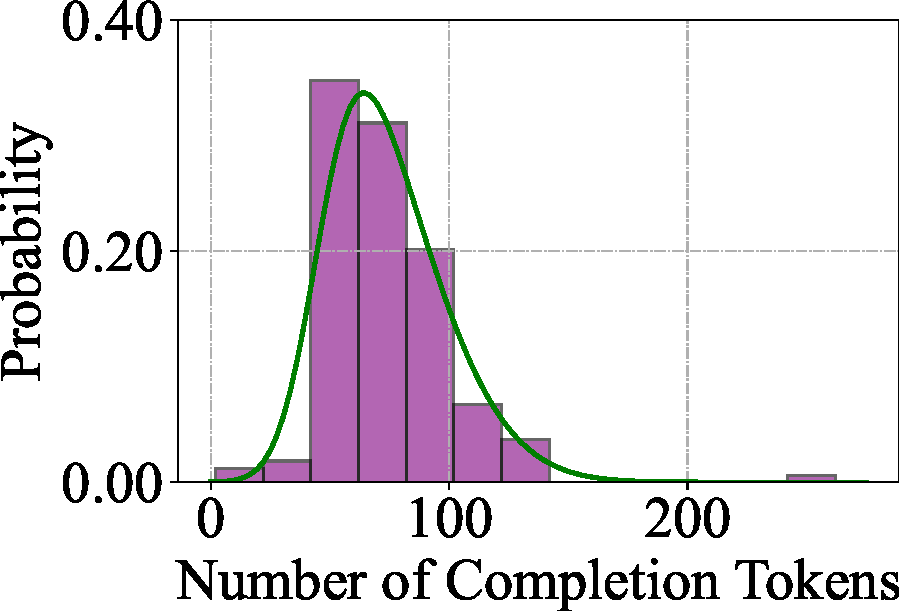
\includegraphics[width=3.2cm]{figures/completion/0.pdf}
			\label{fig:c_token_factoolcode}
		}\hfill
		\subfloat[Document Merging]
		{	
			\centering
			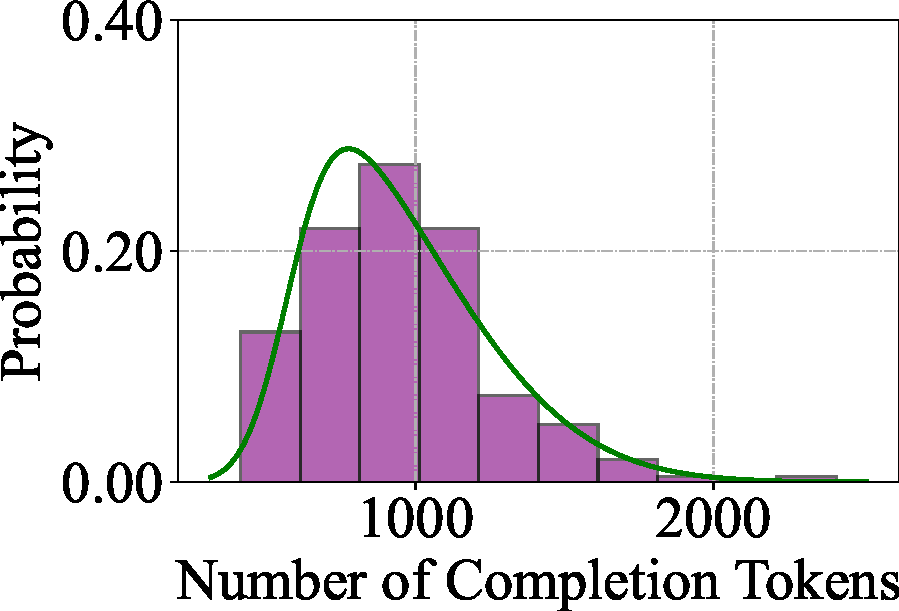
\includegraphics[width=3.2cm]{figures/completion/3.pdf}
			\label{fig:c_token_gotdecmerge}
		}\hfill
		\subfloat[KBQAV]
		{	
			\centering
			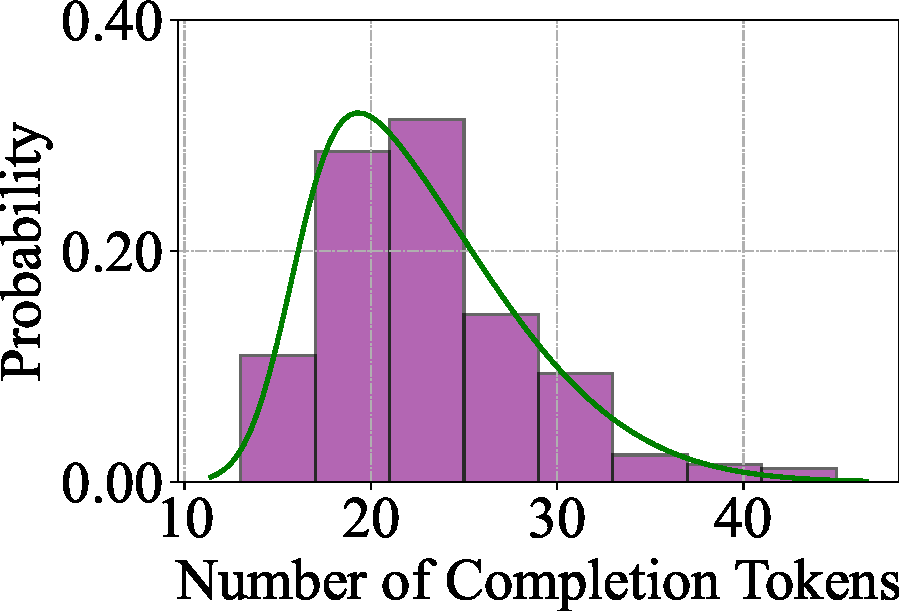
\includegraphics[width=3.2cm]{figures/completion/1.pdf}
			\label{fig:c_token_factoolkbqa}
		}\hfill
		\subfloat[Equation Verification]
		{	
			\centering
			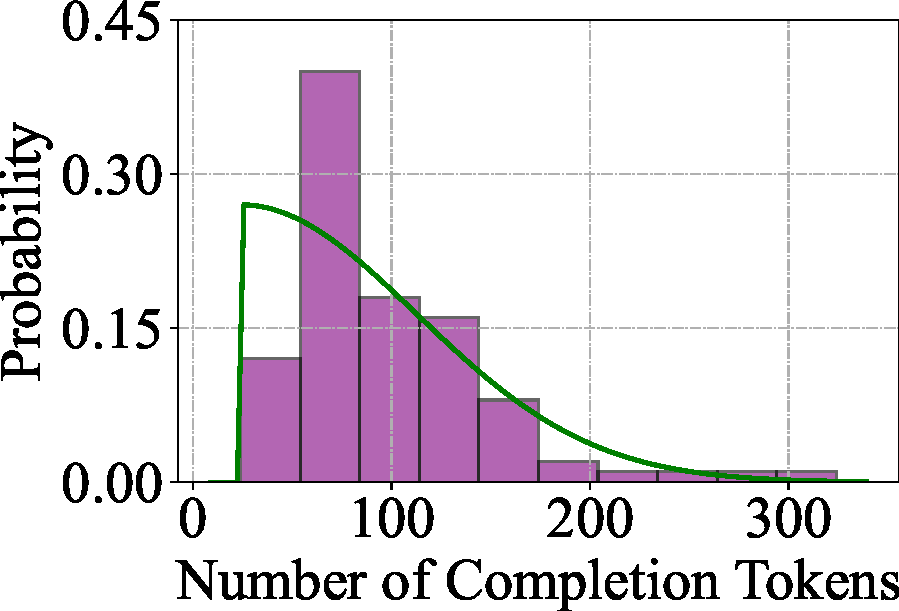
\includegraphics[width=3.2cm]{figures/completion/2.pdf}
			\label{fig:c_token_factoolmath}
		}\hfill
		\subfloat[Fact Extraction and Verification]
		{	
			\centering
			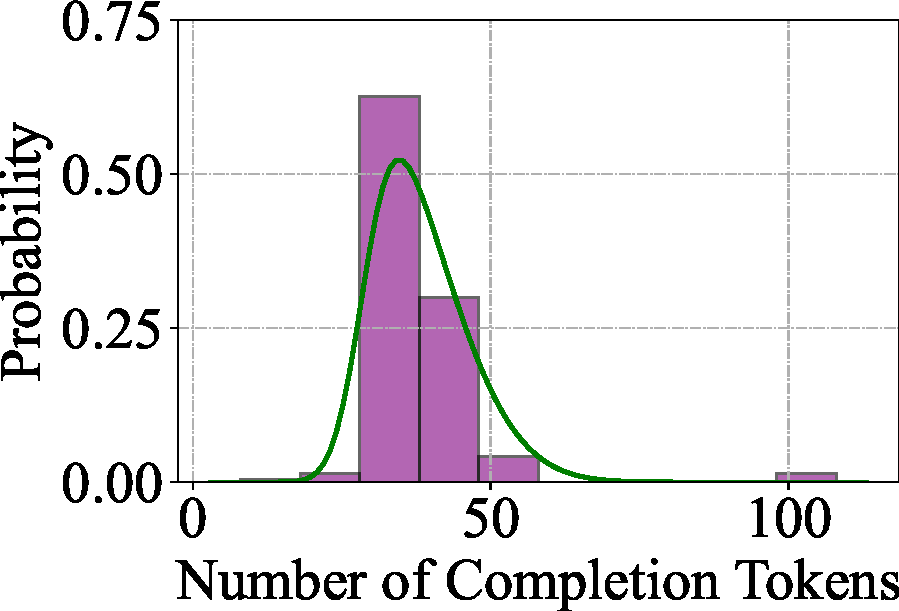
\includegraphics[width=3.2cm]{figures/completion/4.pdf}
			\label{fig:c_token_reactfever}
		}
            \vspace{-.1in}
		\caption{
                Prompt and completion token length distribution for an arbitrarily-selected request (marked at the top) in five applications each over 100 trial runs.
                In each case, we divide the length range into 10 buckets, and calculate the value appearance probability in each bucket (accompanied by the fitted curves assuming skewed Guassian distribution for reference).}
		\label{fig:token_usage}
	}
\end{figure*}


Nonetheless, although those works are application-aware, they largely ignore the three characteristics of LLM applications---by focusing on a single application structure (e.g., text streaming~\cite{liu2024andes}), a single resource type (e.g., KV-cache~\cite{gao2024cost}) or a single scheduling objective (e.g., end-to-end completion time~\cite{lin2024parrot}). 
There is a lack of a serving system designed for general LLM applications with their common characteristics properly handled, which further leads to two consequences.

First, due to the overwhelming demand dynamicity, it is hard to know the application-level resource consumption, rendering it difficult to improve the overall ACT with advanced scheduling algorithms like SRPT (letting alone to smoothly support diverse scheduling objectives).
Second, when serving LLM applications in the dark, it is hard to coordinately provision the desired resources on each backend, and a single LLM application---even when it is prioritized in the global queue---may still be impeded on any backend due to factors like cold cache, non-LLM resource contention and improper backend configuration (detailed later in \S\ref{subsec:resource_provisioning}).

% To summarize, although those works are application-aware, they largely ignore the three characteristics of LLM applications: they focus on a single application structure (e.g., text streaming~\cite{liu2024andes}), a single resource type (e.g., KV-cache~\cite{gao2024cost}) or a single scheduling objective (e.g., end-to-end completion time~\cite{lin2024parrot}). 
% There is a lack of a general serving system for LLM applications which can properly deal with their typical characteristics (dynamic demand structures, hybrid resource backends and diverse performance objectives).
% \chen{add more deficiencies}

% Moreover, as we shown later in Sec.X, request correlation awareness not only allows for scheduling at a coarser granularity, but also provides an opportunity to mitigate demand uncertainty---by referring to execution information of the requests in the previous rounds or even of the requests just-finished in the ongoing round. 
% Existing works fail to capture such opportunities and, when serving requests from general LLM applications, have to act in the dark and usually suffer compromised service quality.

\phm{Objective.}
Motivated by the deficiencies of existing works, our objective in this paper is to leverage request correlations for efficient LLM application serving.
In particular, we seek to (1) improve the overall application scheduling performance involving diverse objectives, and (2) speed up individual LLM applications demanding hybrid resource types. 

%!TEX root = main.tex
\section{\emph{Coinference}: The Demand Abstraction for LLM Applications}
\label{sec:abstraction}


To facilitate efficient serving and demand modeling of an LLM application, we propose the abstraction of \emph{coinference}, which refers to the entire set of LLM inferences within an LLM application.
To better elaborate the concept of coinference, we resort to Fig.~\ref{fig:app_structure}, which shows the execution workflow of a series of representative LLM applications.
As shown in Fig.~\ref{fig:app_structure}, each application involves both LLM (in orange) and non-LLM tasks (in white).
Note that, although an LLM application has hybrid resource demands, our coinference abstraction here sets only the LLM inference requests as first-class citizens: LLM inferences usually take the largest service cost, and meanwhile they are the common parts in all the LLM applications with clear execution patterns (we will show how to integrate the non-LLM resource demands later in \S\ref{subsec:demand_modeling}).

\phm{Feasiblity.} 
We note that the correlations among LLM requests are easy to obtain in practice. 
For example, when a user executes an LLM application by calling the OpenAI assistants API~\cite{assistants_api} (essentially a customized cloud-hosted agent), the OpenAI backend associates all the messages (LLM requests) for that application with a common \emph{thread ID}.
Moreover, the metadata in LLM requests is often flexible to customize---for example, the \texttt{extra\_body} parameter is provided by OpenAI~\cite{OpenAI_extra_body} and vllm~\cite{vLLM_extra_body} to accept additional JSON properties, thus the application affiliation information can be easily integrated into each LLM request.  



\phm{Opportunities.}
As aforementioned, formally adopting the coinference abstraction brings two opportunities on serving enhancement for LLM applications.
First, as showcased in Fig.~\ref{fig:toy_example}, by scheduling the LLM requests at the coinference level (in proper order), we can remarkably improve the overall scheduling performance against diverse application-level objectives. 
Second, coinference-level performance modeling can help more precisely monitor the demand status of each LLM request, which we here verify empirically. 

To elaborate, we run five LLM applications from Fig.~\ref{fig:app_structure} each for 100 times (with different inputs from the original dataset).
Fig.~\ref{fig:token_usage} records the execution statistics in input (prompt) and output (completion) token lengths for an 
arbitrarily selected request of each application.
%In particular, we divide the length range for each request position into 10 buckets, and calculate the probability of each bucket (accompanied by the fitted curves assuming skewed Guassian distribution, for reference). 
As shown in Fig.~\ref{fig:token_usage}, although the resource demands are non-deterministic, they do exhibit salient stability across different trial runs.
%\chen{For example, the input token length of the Document Merging application is always larger than 1000, yet for KBQAV application it is always between 360 and 380. }
For example, the output token length of the \texttt{merge} request in Document Merging application is around 1000, yet for the \texttt{generate-query} request in KBQAV application it is between 10 and 50.
That phenomenon is indeed reasonable because demand volume is to some extent an inner property based on the usage scenario of an LLM application:
the output of the \texttt{merge} request is a document, yet for the \texttt{generate-query} request it is a short query---thus its length distribution has a much smaller mean value and also a much smaller deviation. 
This way, the historical statistics can help to narrow down the estimation range of request demands and facilitate accurate prediction. 
Moreover, as we show later (\S\ref{subsubsec:correlation_analysis}), for requests with dependencies, the upstream requests just-finished can also work as an informative indicator of the demand quantity of downstream requests.
This can further strengthen the effectiveness of coinference-based demand prediction. 

%\phm{Insight and Challenges.}
To summarize, the coinference abstraction---as a scheduling unit as well as a demand predicting approach---makes it quite promising to realize our previous objectives (multi-application scheduling enhancement and single-application processing acceleration).
%However, the coinference abstraction is only a starting point and many challenges still need to be solved to unleash its power in practice.
Note that in the network community, there exists a similar notion, \emph{coflow}~\cite{chowdhury2012coflow,chowdhury2014efficient}, which seeks to group together all the flows of a data analytics job in scheduling, to make better end-to-end performance.
Yet coinference serving is more difficult than coflow serving: for a coflow, the inner structure is simple (in parallel without dependency); the demand quantity (flow size) is often available a priori; the service objective is mostly to minimize coflow completion time; the resource consumption only involves the network backend.
In that sense, we are addressing a brand-new problem where the coinference abstraction is only a starting point.
%only recording the inference correlation is not enough.
Next, we show how to use the coinference abstraction to improve the service quality of LLM applications with their challenging characteristics handled.
% with the objective of making multi-application scheduling enhancement as well as single-application service acceleration.

% We find that the resource demands across coinferences of a given application are similar and typically follow a certain distribution, such as skewnorm. As shown in fig We measured the resource demands of various applications and fitted them to appropriate distributions, allowing us to gain a statistically insight of each application's factors such as stage parallelism, output token length, kv-cache size, time gap, and other factors. This serves as prior knowledge for predicting and scheduling.
%!TEX root = main.tex
% \section{Solution - Hermes}
% \label{sec:solution}

\section{$\!\!\!$Hermes: Coinference-Centric LLM Serving$\!$}


\subsection{Overview}
\begin{figure}
    \vspace{-.1in}
    \centering
    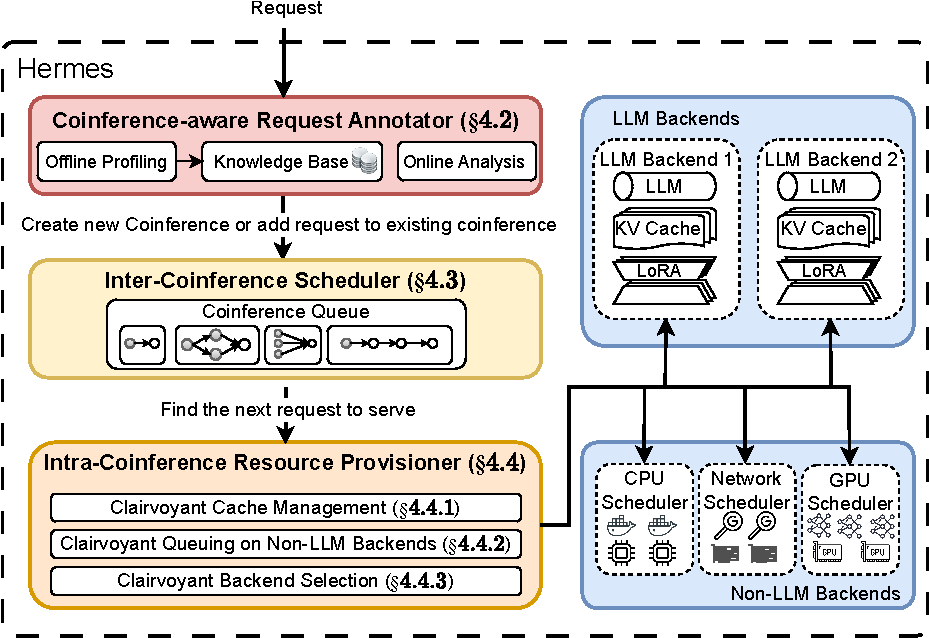
\includegraphics[width=0.95\linewidth]{figures/overview.drawio.pdf}
    \caption{The system architecture of Hermes.}
    \label{fig:overview}
    \vspace{-.2in}
\end{figure}

% Fig.~\ref{fig:overview} provides an overview of Hermes's design. Hermes incorporates a \emph{Coinference-aware Request Annotator} (\S\ref{subsec:demand_modeling}) to model the resource demand required to complete a Coinference. Each incoming request is added to a newly created or existing Coinference based on the information provided by the annotator. Besides, Hermes designs a Coinference-centric Scheduler called \emph{Inter-Coinference Scheduler} (\S\ref{subsec:inter-coinf scheduling}). This scheduler calculates the priority of each Coinference and allocates requests accordingly iteratively. Additionally, to enhance the service of high-priority Coinferences, Hermes includes an \emph{Intra-Coinference Resource Provisioner} (\S\ref{subsec:resource_provisioning}). This component ensures that Coinferences with higher priority receive better service, regardless of whether they involve LLM, Non-LLM, or multiple backend systems.

Based on the above coinference abstraction, in this paper we design Hermes, a coinference-centric serving system for LLM applications. 
Hermes has three key modules as shown in Fig.~\ref{fig:overview}.	
First, there is a \emph{Coinference-aware Request Annotator} (\S\ref{subsec:demand_modeling}) that annotates the coinference-level demand information for each incoming request, so as to facilitate later inter- and intra-application optimizations. 
The demand models are built offline with a series of profiling runs and stored in a knowledge base.
Second, the \emph{Inter-Coinference Scheduler} (\S\ref{subsec:inter-coinf scheduling}) determines the proper scheduling priority of different requests from the coinference-level viewpoint. 
Third, to efficiently execute each individual request, the \emph{Intra-Coinference Resource Provisioner} (\S\ref{subsec:resource_provisioning}) leverages the coinference-level demand information to prepare the desired resources in various aspects: cache management (\S\ref{subsubsec:cache}), queuing management on non-LLM backends (\S\ref{subsubsec:queuing}), and selection of LLM backends with different configurations (\S\ref{subsubsec:selection}). 


\begin{figure}
    \centering
    \begin{minted}[
    frame=none,
    obeytabs=true,
    framesep=0mm,
    baselinestretch=0.9,
    fontsize=\footnotesize,
    xleftmargin=0em,
    breaklines,
    texcomments,
    escapeinside=||
    ]{python}

"application-1":{
    "stage_list":[
        "stage-1":{
            "prompt_tokens": [500, 540,..., 510],
            "completion_tokens": [200, 250,..., 220],
            "request_parallelism": [3, 3,..., 3],
            "loop_times": [2,3,..., 4]
            "next_stage": "stage-2",
            "gap_to_next_stage": [1.2, 1.1, ..., 1.5],
            "demand_during_gap": {
                    "cpu_core": 1,
                    "memory": 2,
                },
            "demand_correlation_mask": (0,1,1,0,1),
        },
        "stage-2":...,
        "stage-3":...,
        ...
    ],
}

    \end{minted}
    \vspace{-0.3cm}
    \caption{An example of coinference demand model.} 
    %The Example of How We Model an Application \chen{describe the meaning?} \gz{For each application, we maintain a stage list that contains the information dictionary for every type of stage of this application. This information dictionary includes the distribution of resource demand (e.g. number of prompt tokens, number of output tokens), the probability of transitioning to every possible next stage, and a mask indicating demand correlation.}}
    \label{fig:demand_model}
\end{figure}


\subsection{Coinference Demand Modeling}
\label{subsec:demand_modeling}

In coinference demand modeling, we seek to panoramically capture the demand characteristics of an LLM application through a series of offline profiling runs. 
Our objective  here is to design a (1) \emph{general} representation method that is applicable to diverse LLM applications and, in the meantime, (2) as \emph{precise} as possible. 

\subsubsection{Towards general demand modeling.}
We first focus on the \emph{generality} aspect. 
To design a general demand modeling method, we need to properly handle the \emph{diversity} and \emph{uncertainty} of LLM applications. 
We will respectively show our solutions in such two aspects with Fig.~\ref{fig:demand_model}.

\textit{1) Handling structure and resource diversity.}
% First, different coinferences have their constituting LLM requests organized in different structures. 
% To be specific,
In typical LLM applications, there are heterogeneous relationships among the requests of a coinference: some requests are in parallel with each other,
%(e.g., for those in the summary-chunks phase in Fig.~\ref{fig:app_structure}(h)), 
whereas some others have rigid dependencies. % (e.g, for those across the generate and score phases in Fig.~\ref{fig:app_structure}(c)).  
To describe such diverse request relationships in a general manner, we adopt a \emph{stage-centric} paradigm.
An LLM application usually contains a series of functional units---each issuing one or multiple parallel inferences that are submitted almost concurrently and also share the \emph{same system prompt}; such a functional unit is defined as a \emph{stage}\footnote{
    The stage affiliation of a request can be manually annotated by the \texttt{extra\_body} parameter (as the application affiliation) or automatically detected by analyzing the prompt prefix.
}.
%At online serving time, the stage affiliation of a request can be easily identified from its prompt.} 
Therefore, we can organize the requests of a LLM application as a list of stages; each stage records the request-level demand (input/output token length) and also maintains a \texttt{next\_stage} property to record the dependency information.
% As shown in Fig.~\ref{fig:demand_model}, each stage maintains the \texttt{next\_stage} property to record the dependency information. 
% \chen{and we sketch the LLM resource demand (prompt token, completion token, parallism) based on the constituting requests.}
Second, executing an LLM application also requires diverse resource backends like CPU and network (for tool calling); such non-LLM resources are usually consumed  during the gaps between LLM inferences.
To express such non-LLM resource demand, we incorporate the consumption amount (e.g., 1 cpu core and 2GB memory) as well as the gap length to the dependency information, as expressed by the \texttt{gap\_to\_next\_stage}\footnote{
For LLM applications without tool calling (e.g., for Chatbot), \texttt{gap\_to\_next\_stage} can also be leveraged to represent the typical interaction pace incurred by factors like network transmission delay. 
} and \texttt{demand\_during\_gap} properties in Fig.~\ref{fig:demand_model}.

\textit{2) Handling structure and request-level uncertainty.}
Demand uncertainty (i.e., runtime dynamicity) means that an LLM application has different stage structures or demand quantities in different execution rounds.
% that the demand pattern of an LLM application usually fluctuates across different execution rounds, which may occur in various aspects: the stage structure,
%(for applications with ReActing and LLM-planning), 
%the request parallelism,
%(if not predefined but determined by inputs), 
%as well as the request input/output token length.
% Such variations need to be comprehensively expressed to facilitate future demand prediction.
Structural uncertainty is mainly caused by the looping LLM requests in ReActing-like applications\footnote{
We admit that plan-and-execute applications may also yield dynamic structures, which is difficult to address given the diverse functional units after planning. 
For consistent modeling with reasonably good performance, we dictate that each plan-and-execute application always has two stages---a \emph{planning} stage and an \emph{executing} stage. % , which can facilitate consistent modeling with reasonable good performance. 
In that sense, a N-step-after-planning application would have an \emph{executing} stage that loops for N times. 
}.
To build a stable application structure despite such looping dynamicity, we introduce the \texttt{loop\_times} property in each stage to describe its looping status across different profiling rounds.
Moreover, when expressing the quantity variation in each demand aspect (input/output token length, request parallelism, loop times and post-stage gap), we choose to 
%To express stage structure variation, we resort to a \emph{probability-graph-like} strategy: given that a stage may have multiple downstream branches (sometimes may looping to itself), we associate a \texttt{frequency} property to each downstream stage. 
% To express request parallelism variation, we choose to 
directly append the raw value profiled from each trial run to a list. 
We note that recording the raw values is better than recording the coefficients of the fitted skewed norm distribution, considering the depiction fidelity (the true distribution is in fact irregular) and computation efficiency---it takes much time (up to seconds) to fit out the coefficients as well as to support our later calculations (e.g., correlation analysis and integral calculus).
In practice, we set the maximal length of the recorded value list to $500$ (evicted in FIFO manner), and the storage cost is indeed negligible on cutting-edge GPU servers. 
% (fitting ou\footnote{
%     %We note that recording the raw values is better than recording the coefficients of the fitted skewed norm distribution shown in Fig.~\ref{fig:token_usage}: although the later is more concise, it is however not appropriate for our use.
%     First, there are still error gaps between the true distribution and the skewed norm distribution;
%     second, such an analytic method is not computation-efficient---it takes much time (up to seconds) to fit out the coefficients as well as to support our later calculations (e.g., correlation analysis and integral calculus).
%     %and applying them for our later integral operations (Sec. X) are computation-inefficient---taking even seconds with the \chen{XX lib}. 
%     In contrast, recording the raw data is computation-efficient, and the storage cost (we set a maximal record number $500$) is indeed negligible on cutting-edge GPU servers. 
% }.
% To express input/output length variation, we also record the raw data in a list. 
%Note that we additionally record the inter-stage time gaps---which may also vary across different rounds---in the same manner with raw data stored in list. 
%Moreover, we also record the execution time of the entire LLM application by summing up all the stage durations and gaps.
%\chen{some details unclear: multiple request? how to use mean and deviation?}

% \begin{figure*}
% 	\parbox[t]{18cm}{
% 		\centering
% 		{	
% 			\centering
% 			
\includegraphics[width=3.2cm]{figures/gap/1.pdf}
% 			\label{fig:gap_factoolkbqa}
% 		}\hfill
% 		{	
% 			\centering
% 			
\includegraphics[width=3.2cm]{figures/gap/4.pdf}
% 			\label{fig:gap_gotdocmerge}
% 		}\hfill
% 		{	
% 			\centering
% 			
\includegraphics[width=3.2cm]{figures/gap/2.pdf}
% 			\label{fig:gap_reactfever}
% 		}\hfill
% 		{	
% 			\centering
% 			
\includegraphics[width=3.2cm]{figures/gap/3.pdf}
% 			\label{fig:gap_reactalfw}
% 		}\hfill
% 		{	
% 			\centering
% 			
\includegraphics[width=3.2cm]{figures/gap/5.pdf}
% 			\label{fig:gap_langchainmapreduce}
% 		}\hfill
% 		{
% 			\centering
% 			
\includegraphics[width=3.2cm]{figures/duration/2.pdf}
% 			\label{fig:duration_factoolkbqa}
% 		}\hfill
% 		{	
% 			\centering
% 			
\includegraphics[width=3.2cm]{figures/duration/1.pdf}
% 			\label{fig:duration_gotdecmerge}
% 		}\hfill
% 		{	
% 			\centering
% 			
\includegraphics[width=3.2cm]{figures/duration/4.pdf}
% 			\label{fig:duration_reactfever}
% 		}\hfill
% 		{	
% 			\centering
% 			
\includegraphics[width=3.2cm]{figures/duration/5.pdf}
% 			\label{fig:duration_reactalfw}
% 		}\hfill
% 		{	
% 			\centering
% 			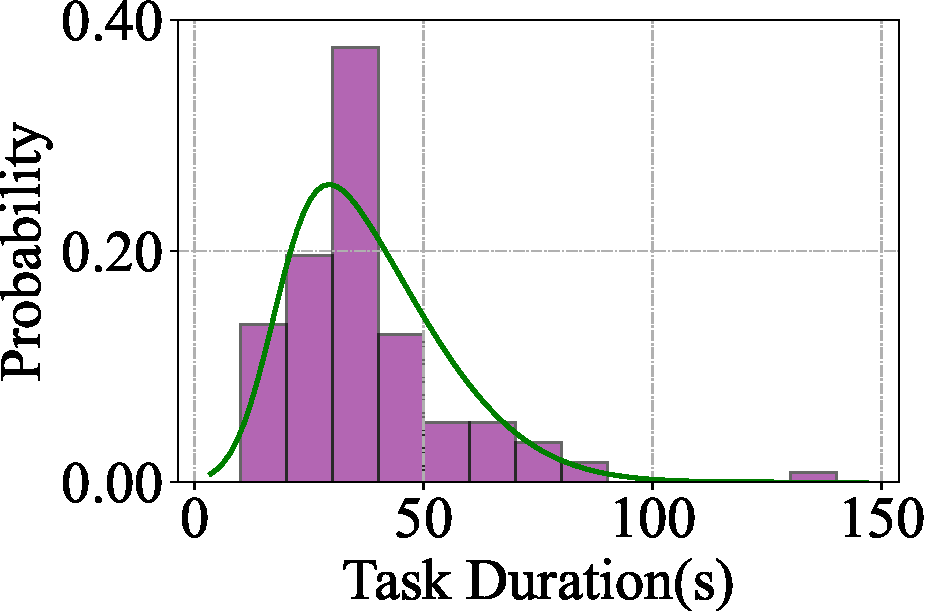
\includegraphics[width=3.2cm]{figures/duration/6.pdf}
% 			\label{fig:duration_langchainmapreduce}
% 		}\hfill
% 		\subfloat[FacTool kbqa]
% 		{
% 			\centering
% 			
\includegraphics[width=3.2cm]{figures/requestnum/0.pdf}
% 			\label{fig:requestnum_factoolkbqa}
% 		}\hfill
% 		\subfloat[GoT docmerge]
% 		{	
% 			\centering
% 			
\includegraphics[width=3.2cm]{figures/requestnum/5.pdf}
% 			\label{fig:requestnum_factoolmath}
% 		}\hfill
% 		\subfloat[ReAct fever]
% 		{	
% 			\centering
% 			
\includegraphics[width=3.2cm]{figures/requestnum/2.pdf}
% 			\label{fig:requestnum_reactfever}
% 		}\hfill
% 		\subfloat[ReAct alfw]
% 		{	
% 			\centering
% 			
\includegraphics[width=3.2cm]{figures/requestnum/3.pdf}
% 			\label{fig:requestnum_reactalfw}
% 		}\hfill
% 		\subfloat[LangChain mapreduce]
% 		{	
% 			\centering
% 			
\includegraphics[width=3.2cm]{figures/requestnum/4.pdf}
% 			\label{fig:requestnum_langchainmapreduce}
% 		}
% 		\caption{Gap Time, Task Duration and Number of Requests in Applications.}
% 		\label{fig:request_num}
% 	}
% \end{figure*}


% We are committed to developing a demand representation method for general LLM applications, capable of providing a comprehensive view of the app's execution process. By "comprehensive," we mean having a sufficient understanding of the app's requirements at both the coinference and stage levels, enabling effective coinference-level scheduling and resource provisioning.
% To achieve the above goal, we plan to approach Coinference Demand Modeling from two aspects: structure and demand.

% However, the greatest challenge lies in how to guarantee the precision and generality of the model when the modeling object is dynamical.
% The dynamics in structure primarily is because: within coinference, some stages exhibit dynamic changes in parallelism, and there are conditional jumps between stages, leading to structures such as loops and branches. Additionally, different coinferences may have significantly different structures due to design variations, as shown in Figure 1. With the ongoing development of LLM applications, even more diverse structures are expected to emerge.
% In terms of resource demands, the differences are even more pronounced. For LLM stages, we cannot know the length of decoding for each request, and the inputs and outputs of each stage are interrelated, making the execution process of coinference highly uncertain. In non-LLM stages, there may be calls to an expanding array of tools, which in turn rely on various traditional backend resources such as CPU and network bandwidth.
% Our goal is to include both existing and future potential structures and demands in our modeling framework, but this presents significant challenges.
% \subsubsection{Modeling for General and Complex Structure}


% To better harness LLM's potential in text analysis, problem-solving, and related areas, there is a growing trend toward dividing a complex application into what we call \textbf{Stages}, in which multiple LLM inferences are conducted with different prompts and Tools(like python, wiki...) are used to help generate LLM prompts containing different implications. This method succeed in improving LLM's performance, especially in complex application. We 
%  divide these applications that triggers multiple LLM inference into three categories according to structure pattern, and carry out a survey on demand aspects, which will be shown at 3.? in details.

% \textbf{Static Pipeline \& Static Parallelism:} in this kind of structure patterns,  the conduct order of stages and the parallelism of LLM requests in each stage are static. We take Factool\_code, Got\_docmerge for examples.   

% Factool\_code is an application provided by Factool to examine the factuality of the code generated for corresponding question. As shown in \ref{fig:factool_code_structure}, given the question and code answer, we first request LLM service to got several testcases, then we use LLM to generate another 3 solutions to the given question, after execute all the 4 solutions using python tool, we compare the result we get, if consistent, the code is factual.


% Got\_deocmerge is an application provided by Got to merge four documents into one. As shown in fig??, Got define a graph of operations, in which nodes represent the current state, while edges represent operations, so pipeline is static. The out-degree represent the parallelism of corresponding operation, whether using LLM or not, which is static too. With a stack-like controller, got is conduct in BFS order. 

% % First, we generate 5 possible result originating from initial state, then score them with the help of LLM and keep the best 3, after that we combine the best 3 in stage aggregate and generate 5 new node, score again and  only keep the best 1, originating from that generate 10 solutions, select the best as result.

% \textbf{Static Pipeline \& Dynamic Parallelism:} in the kind of structure pattern, pipeline is also static, but in some stages the parallelism of LLM requests varies between Coinferences. We take Factool\_kbqa, Factool\_math for example.

% Factool\_kbqa is an application in Factool to examine the factuality of a question-answer pair. As shown in fig??, we first ask LLM to conclude all claims contained in the answer, then generate particular queries that could justify the turth of each claim, therefore the parallelism of the stage query\_generation is up to how many claims attained in stage claim\_generation, which varies when input changes. For each query, we search it on wiki, this stage demand no LLM resource and lead into gap between LLM inference. In verify stage, we ask LLM to distinguish whether the wiki-search result support the corresponding claim, the parallelism of this stage is consistent with stage query\_generation. If all claims supported, the question-answer pair is factual.

% Factool\_math is similar to Factool\_kbqa, while in Factool\_math, inputs are math problem and its answer, claims represent every  calculate in the answer, queries are pieces of python code which could do the calculates in claims, after execute python calculate instead of wiki search, we could verify the truth of each claim without LLM in this application. The parallelism of stage query\_generation is dynamic, because the num of claims is not sure.  

% \textbf{Dynamic Pipeline:} in this kind of structure pattern, some stage's 
% successor have more than one selections, so they don't have fixed pipeline with single direction. Stages' parallelism could be dynamic too theoretically, but not usual in current applications. We take react\_fever, react\_alfw for examples.

% React\_fever and React\_alfw are applications of react in FEVER (Fact Extraction and Verification) and ALFWorld (Action Learning From the Web). As shown in fig??, stages alternate between think and action, the environment take actions guided by LLM response in think stage, return the observation (google-search result in React\_fever or text-world changes in React\_alfw), which will be added into prompt of next think stage.

% In all applications above, users are mainly concerned about the whole conduct time instead of time duaration of each single stage. We conduct measurements on both whole task time and stages' demand, table?? show their type and range of the dataset. fig?? show the task\_time distribution of different applications, the difference between them make it possible to predict and perform SJF scheduling.

% \begin{table}[htbp]
%     \centering
%     \begin{tabular}{|c|c|c|c| }
%         \hline
%         application & Pipeline & parallelism & size of dataset \\ \hline
%         Factool\_code & Static  & Static  & 164 \\ \hline
%         Got\_docmerge & Static & Static  & 100 \\ \hline
%         Factool\_kbqa & Static & Dynamic & 256 \\ \hline
%         Factool\_math & Static & Dynamic & 100 \\ \hline
%         React\_fever & Dynamic & Static & 105 \\ \hline
%         React\_alfw & Dynamic & Static & 95\\ \hline
%         Mapreduce & Dynamic & Dynamic & 112 \\ \hline
%     \end{tabular}
%     \caption{basic information of applications under conduct}
%     \label{tab:agent_list}
% \end{table}

% \begin{figure}[htbp]
%     \centering
%     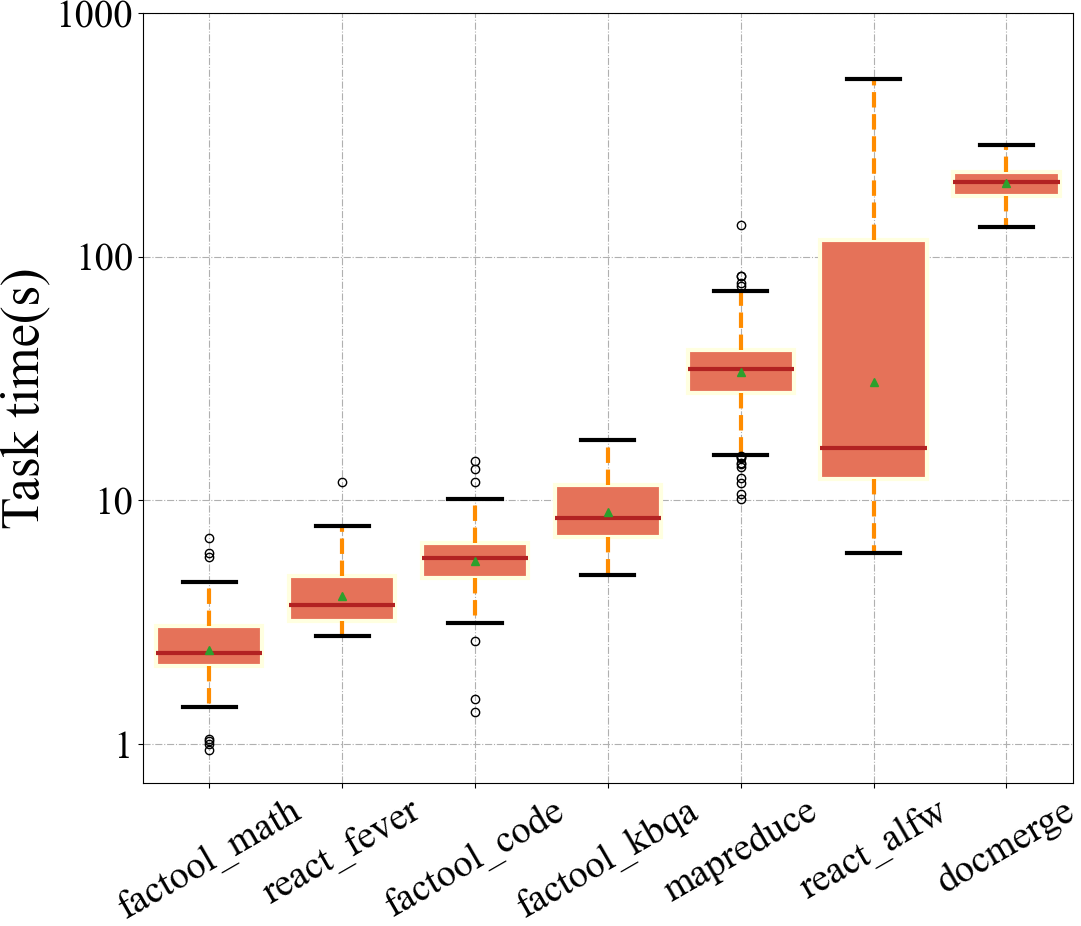
\includegraphics[width=\linewidth]{figures/box.png}
%     \caption{The box plot of coinference time of applications}
%     \label{fig:time_task_all}
% \end{figure}


% \subsubsection{Modeling for Rich and Scalable Attributes}

% \yfliu{During the life cycle of a coinfer, it can be in one of three states: UnFinished, Stage-Finished, or Coinference-Finished.}

% \begin{figure}[t]
%     \centering
%     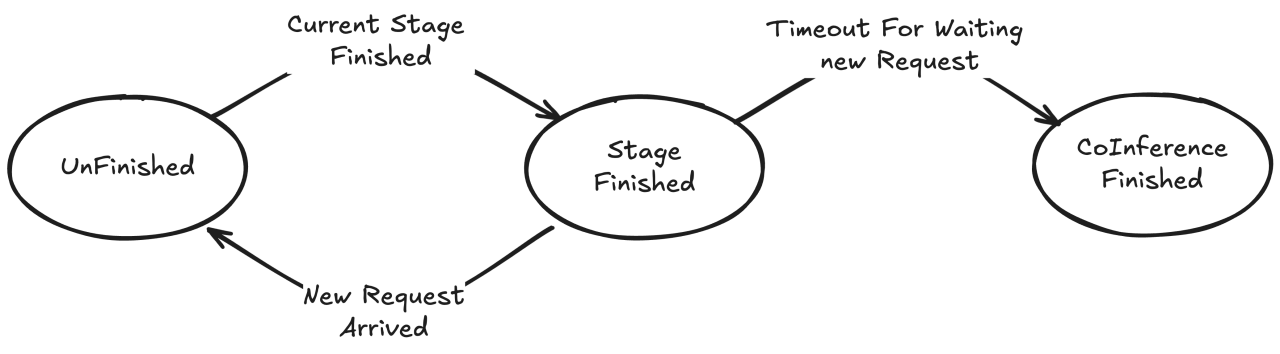
\includegraphics[width=1\linewidth]{figures/state_machine.png}
%     \caption{state machine}
%     \label{fig:state_machine}
% \end{figure}

% We use histograms to describe the distribution of various stage attributes, such as gap duration, number of parallel requests, prompt length, output length, and the transition probabilities to next stages (mainly the times it may loop).

\subsubsection{Towards precise demand modeling.}
\label{subsubsec:correlation_analysis}

Note that the ultimate purpose of demand modeling is to support accurate demand prediction at runtime. 
So far, we have made that by creating a general stage demand portrait from the past execution rounds.
Apart from such cross-round hints, we can future enhance the prediction accuracy by correlation hints in the ongoing round.
Due to the structural dependencies among stages, the resource demands of a stage are often correlated to the upstream ones. 
We note that there typically exist three cross-stage\footnote{
    For simplicity, we assume a Markov model in correlation analysis and only consider the correlation between directly dependent stages.
    }
demand correlation patterns:

    \emph{1)} A stage's request input length may be correlated to the upstream stage's request input length and output length.
        For example, for the Document Merging application, the input of each request in the \emph{scoring} stage is a superset of a request's output in the (upstream) \emph{aggregate} stage (plus a fixed system prompt). 
        Meanwhile, for the looping stages, downstream requests would share the same prompt template as the upstream ones, indicating similarity in input length.
    \emph{2)} A stage's request output length may be correlated to its input length as well as the upstream stage's request output length.
	% Note that the input and output length might be correlated in some cases.
	For example, for the \emph{generate-code} stage in Code Checking application, a more complex input task (often with a longer prompt) usually yields a longer code segment; so for other LLM-tasks like translation and article correction/polishing.
	Meanwhile, for the looping states, the request output lengths are also similar across stages.
    \emph{3)} A stage's request parallelism may be correlated to the upstream stage's request parallelism. 
	For example, as shown in KBQAV applications, for each inference request in the (upstream) \emph{generate-queries} stage, a corresponding inference request would be launched at the (downstream) \emph{verify-claim} stage.

\begin{figure}[t]
	\centering
	\vspace{-0.1in}

    \subfloat[KBQAV]
    {	
        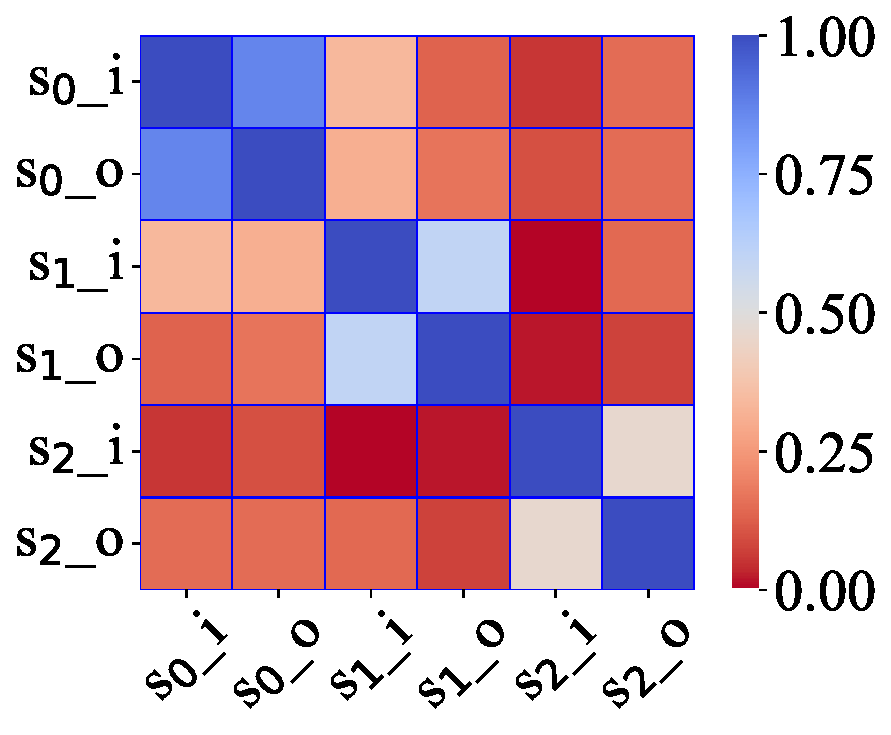
\includegraphics[width=0.45\linewidth]{figures/heatmap_kbqa.pdf}
        \label{fig:heatmap_kbqa}
    }  
    % \subfloat[Math\_FacTool]
    % {	
    %     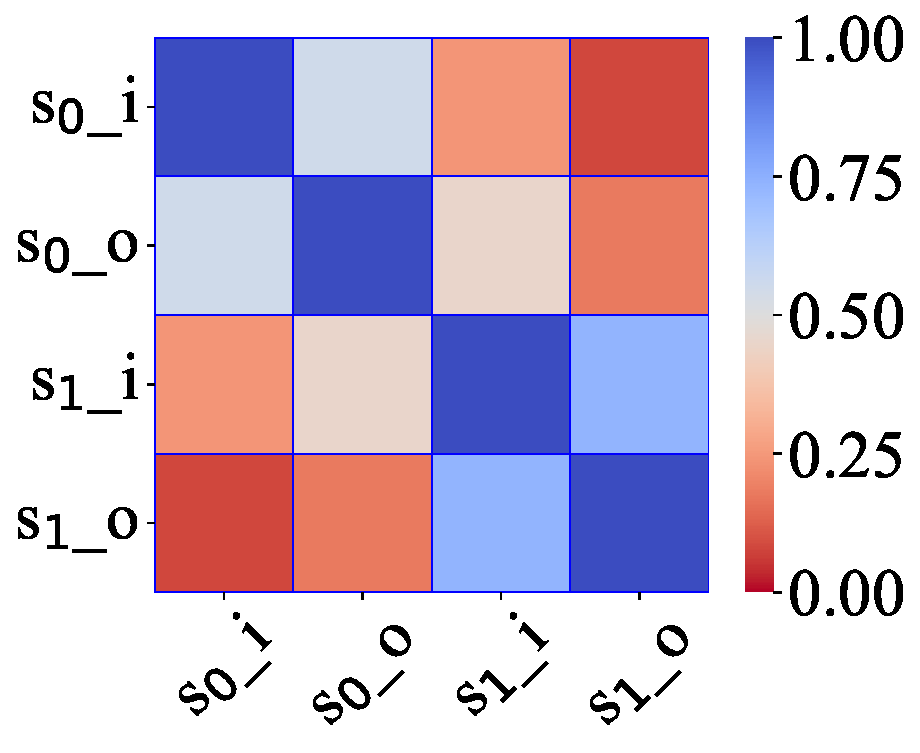
\includegraphics[width=0.2\linewidth]{figures/heatmap_math.pdf}
    %     \label{fig:heatmap_math}
    % }
    \subfloat[Document Merging (DM)]
    {
        \label{fig:heatmap_docmerge}
        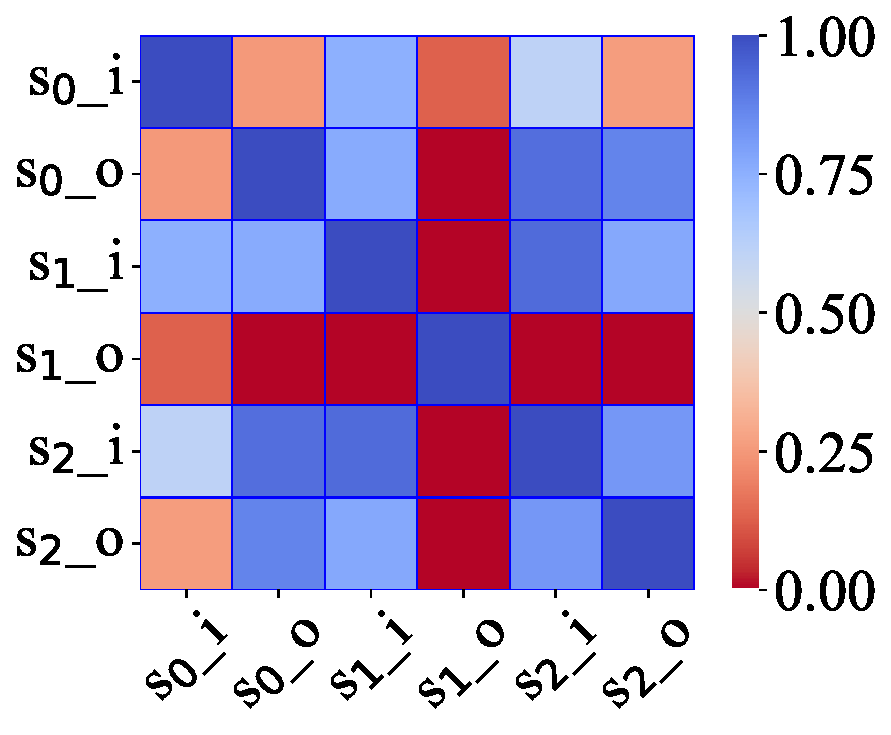
\includegraphics[width=0.45\linewidth]{figures/heatmap_mapreduce.pdf}
    }    
	\vspace{-0.05in}
	\caption{The Pearson correlation coefficients between input/output token lengths of different stages. We present the first three stages of KBQAV and DM, where $s_x$\_$i$ and $s_x$\_$o$ represent the input and output token length of the $x$-th stage.
        }
	\vspace{-0.1in}
	\label{fig:heatmap}
\end{figure}

To verify the existence of above correlation types (especially the first two), we resort to Pearson Correlation Analysis~\cite{sedgwick2012pearson} based on our profiled data over 100 trial runs.
We also divide the demand range to 10 buckets (as in Fig.~\ref{fig:token_usage} for ease of analysis), and use $P(X=i) (i=0,1,…,9)$ to represent the probability that the demand quantity variable X falls into bucket-$i$.
Then we calculate the Pearson correlation coefficient between two demand variables X and Y as
% Although modeling revealed that the input and output lengths of LLM requests approximate a skewed distribution, tending to cluster around the mean, the above experiments indicate that relying solely on the offline profile's mean is insufficient to achieve satisfactory prediction accuracy. Therefore, we aim to incorporate an online updating mechanism. Additionally, during the experiments, it was observed that the input and output lengths of different stages are directly or indirectly related. For instance, in React-style tasks, the output from one stage is directly added to the input of the next, leading to a growth trend in inputs. Similarly, in document merge tasks, longer inputs at the beginning often result in longer inputs and outputs in subsequent stages. We measured the correlation between stages of two applications using the Pearson correlation coefficient and represented it with the heatmap Figure \ref{fig:heatmap}. From the visualization results, it is evident that there is indeed a correlation between the inputs and outputs of certain stages within the app. Thus, we introduce Bayesian networks to learn such relationships. 
$\rho_{X,Y} = \frac{\text{cov}(X,Y)}{\sigma_X \sigma_Y} = \frac{\mathbb{E}((X - \mu_X)(Y - \mu_Y))}{\sigma_X \sigma_Y}.$	
In Fig.~\ref{fig:heatmap}, for KBQAV and Document Merging, we further depict the Pearson correlation coefficients between any two demand variables (each represent the input/output length of a stage).
For KBQAV, each stage's output length is strongly correlated to its input length; yet for Document Merging, each stage's input length is highly-related to the upstream stage's input length. 
Fig.~\ref{fig:heatmap} also suggests that each application has distinct correlation patterns; for prediction efficiency, we only consider the demand correlations with a coefficient ($\rho$) larger than 0.5.
To that end, in each stage we add a five-tuple $({M_I^\tilde{I}}, {M_I^\tilde{O}}, {M_O^\tilde{O}}, {M_O^I}, {M_P^\tilde{P}})$ to mask whether the corresponded demand correlation holds: $M_B^A$ represents whether the demand variable $A$ affects $B$; $I$, $O$ and $P$ ($\tilde{I}$, $\tilde{O}$ and $\tilde{P}$) respectively represents the input length, output length and request parallelism of the current (upstream) stage.

The above correlation analysis enables more precise online demand prediction.
Upon the completion of a stage, its execution information can be immediately adopted for demand prediction of the next stage. 
In that case, we are facing a \emph{conditional prediction} problem.
Suppose the request input and output length of the just-finished stage is respectively in bucket $i$ and $o$---with both correlated with the input length of the downstream stage, and we need to predict $P(I|\tilde{I}=I, \tilde{O}=o)$. 
To accomplish that, we join the historical execution records of the two stages (i.e., yielding $(\tilde{I}, \tilde{O}, I)$ tuples respectively from each trial round), and filter out the profiled tuples satisfying $\tilde{I}=i$ and $\tilde{O}=o$; then the $I$ distribution within the filtered records is a more precise prediction for the current round.

% For applications with a Directed Acyclic Graph (DAG) structure, we model each stage’s inputs and outputs across consecutive stages and establish links between each stage and its subsequent stages, forming a Bayesian network for inference. As co-inference proceeds, we sequentially obtain information from each stage, which allows us to make continuously refined predictions for the subsequent stages.Let $ \mathbf{X}_1, \mathbf{X}_2, \dots, \mathbf{X}_n $ be the random variables representing each stage in an application and $ \mathbf{X}_\text{prev} = \{ \mathbf{X}_1, \mathbf{X}_2, \dots, \mathbf{X}_{k-1} \} $ be the variables prior to stage $\mathbf{X}_k$, $ x_\text{prev} = \{ x_1, x_2, \dots,x_{k-1} \}$ presents execution information from previous stages. The conditional probability distribution(CPD) could be represented as equation \ref{eq:bayes cpd}. 

% \begin{equation}
%     P_\text{app}(X_h \mid \mathbf{X}_{\text{prev}} = x_{\text{prev}}) \quad k\leq h\leq n 
% \label{eq:bayes cpd}
% \end{equation}

% For non-DAG applications, especially those with cyclic units, we internalize the concepts of Bayesian maximum likelihood and probability updating. During online execution, we incorporate the encountered input and output results into the offline collected samples and use maximum likelihood methods to predict potential values of the next stage.Let $\{ x_k^{(0)},x_k^{(1)},\dots,x_k^{(m)}\}$represent all possible values of $\mathbf{X}_k$ after discretization. Let $P_{\text{init}}$ and $P_{\text{updated}}$ represent the initial distribution and the updated distribution, respectively. $\mathbf{X}_k = x_k^{(\text{obs})}$ represents the actual observed result for stage $\mathbf{X}_k$. Equation \ref{eq:cpd updated}, \ref{eq:cpd normalize} illustrates how the probability distribution is updated in response to the observed values.

% \begin{multline}
%     P_{\text{updated}}(\mathbf{X}_k = x_k^{(i)}) = (1 - w) P_{\text{init}}(\mathbf{X}_k = x_k^{(i)}) \\
%     + w \cdot \mathbf{sgn}(x_k^{(i)} = x_k^{(\text{obs})})    
% \label{eq:cpd updated}
% \end{multline}

% \begin{multline}
%     P_{\text{updated}}(X_k = x_k^{(i)}) \leftarrow \frac{P_{\text{updated}}(X_k = x_k^{(i)})}{\sum_{j} P_{\text{updated}}(X_k = x_k^{(j)})}
% \label{eq:cpd normalize}
% \end{multline}

% Based on the probability distribution adjusted by the execution results, we can predict the information of following stages more exactly. Due to our two methods, our prediction becomes applicable to a broader and more general range of scenarios. Figure \ref{fig:bayes effect} illustrates the results after adding Bayesian predictions.
% \begin{figure}[htbp]
%     \centering
%     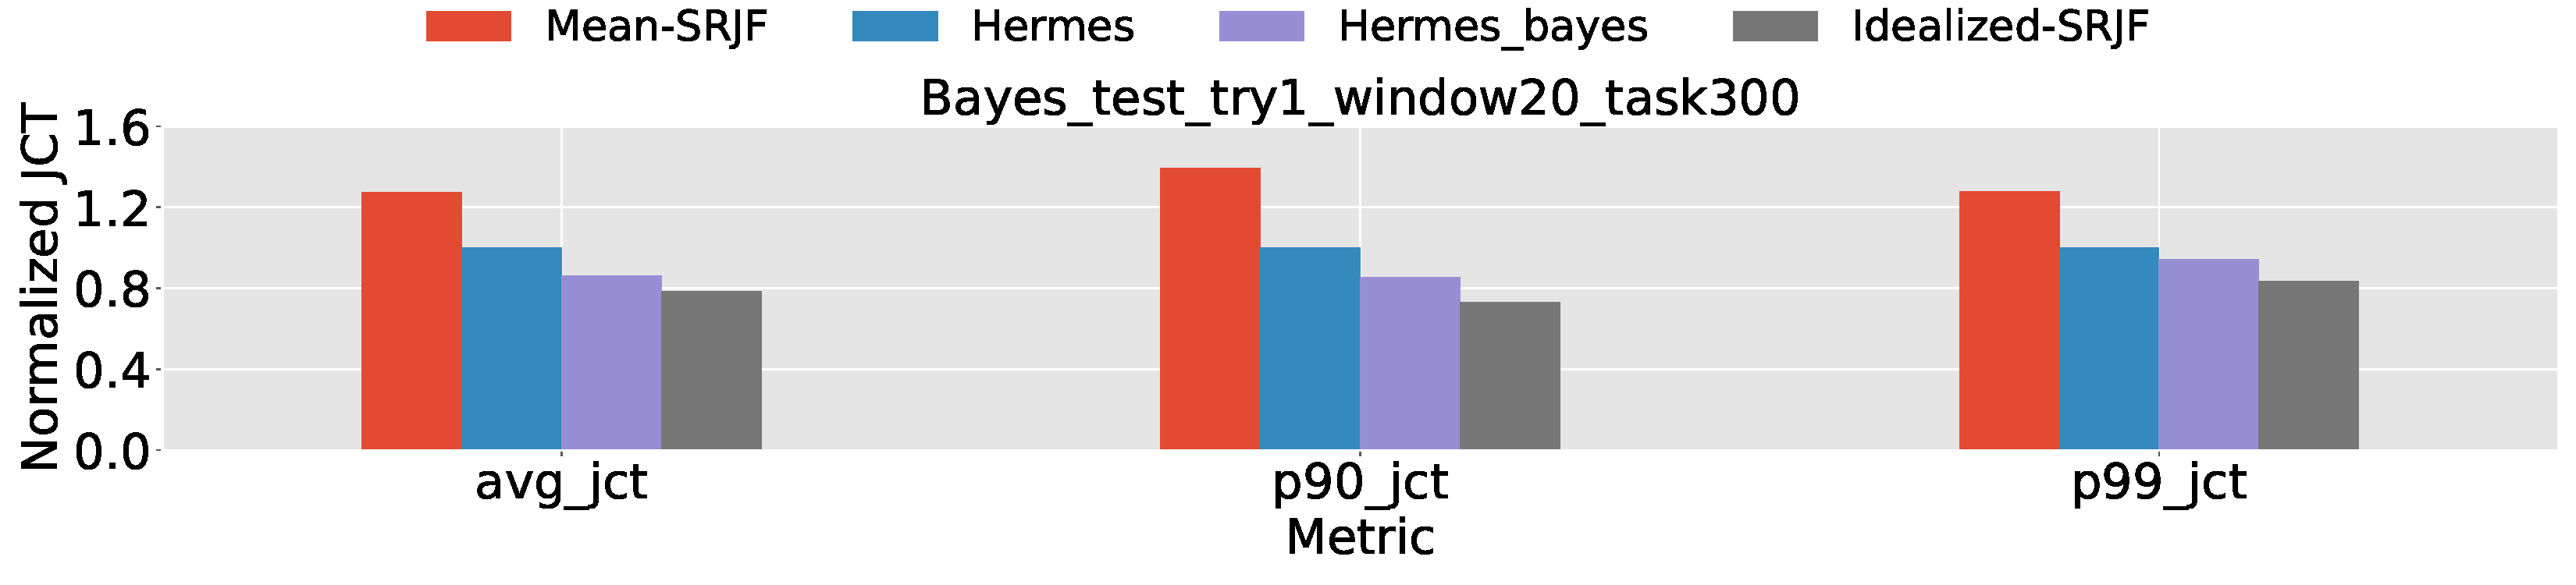
\includegraphics[width=\linewidth]{figures/bayes_mean.pdf}
%     \caption{Comparison of overall execution performance differences across various prediction methods.}
%     \label{fig:bayes effect}
% \end{figure}


\subsection{Inter-Coinference Scheduling}
\label{subsec:inter-coinf scheduling}

As previously showed in Fig.~\ref{fig:toy_example}, the conference abstraction provides us with a high-level scheduling handle.
%  which can effectively support high-level scheduling objectives.  
In this part, we explore how to leverage the coinference modeling results to optimize the inter-coinference scheduling performance.
There are two specific challenges. 
First, how to leverage the distribution-style demand description for scheduling efficiency optimization?
Second, how to deal with the cases where the competing LLM applications have heterogeneous service objectives?
We next address them respectively.

% Most existing LLM inference frameworks, such as vLLM~\cite{}, lack awareness of higher-level application requirements, resulting in interleaved servicing of multiple applications, which can significantly increase latency on the application side. Parrot~\cite{} recognized this challenge and addressed it by jointly scheduling related requests. However, in mixed workloads, it may still experience head-of-line blocking due to large jobs. In this section, we demonstrate how to efficiently schedule various requests at the Coinference level using a Gittins index policy, while also providing service-level-objective (SLO) compliance like deadlines (DDL) and time-per-token (TPT).

\subsubsection{Efficient coinference scheduling with Gittins policy.}
\label{subsubsec:gittins}
We first focus on optimizing the average application completion time. 
A classical algorithm proven optimal in that regard is shortest-remaining-processing-time (SRPT)~\cite{schrage1968proof}, which sets the priority of each request based on the remaining processing time of its coinference.
However, naively applying SRPT is not appropriate for our problem: SRPT relies on deterministic demand values to make scheduling decisions, yet the resource demands of LLM applications in various aspects are usually uncertain a priori (our prior modeling strategies only mitigate but not eliminate such uncertainties). 
Although it is possible to use the expected value (mean) of a demand distribution to emulate SRPT scheduling, this method often fails to work well due to its blindness to instantaneous execution progress.		
For example, for a request with an expected output length of 20 tokens, it is possible that its token generation process does not stop even after 100 tokens.
In that case, we need to timely refresh the demand estimation based on the latest progress rather than sticking to the prior expectations (otherwise the remaining processing time---the expected execution time minus the executed time---may ironically become negative). 
Therefore, we need to introduce uncertainty-awareness in designing our scheduling algorithm.

The problem we now face---minimizing the average completion time for jobs with \emph{unknown durations} but \emph{known duration distributions}---has been well studied in the literature, for which the \emph{Gittins} policy~\cite{gittins2011multi, aalto2009gittins, scully2021gittins} has been proven optimal.
The basic idea of Gittins policy is to calculate a \emph{Gittins rank} for each job---based on its executed time so far and its size distribution---as the scheduling priority.
Specifically, let a request's output length distribution be $\mathcal{D}$, and suppose $a$ tokens have already been generated,
% First, we calculate the Gittins index $g_{output}$ for the output length of each request within the coinference. 
% Let the output length distribution of a request be $d$, and suppose $a$ tokens have already been generated. 
then its Gittins rank $G$ can be expressed as:
% \begin{equation}
% \label{eq:gittins_output}
%     \begin{aligned}
%     G(\mathcal{D},a) = \operatorname*{sup}_{\Delta>0}{\frac{\operatorname*{P}\{X_{\mathcal{D}}-a\leq\Delta\mid X_{\mathcal{D}}>a\}}{\operatorname{E}[\operatorname*{min}\{X_{\mathcal{D}}-a,\Delta\}\mid X_{\mathcal{D}}>a]}},
%     \end{aligned}
% \end{equation}
\begin{equation}
\label{eq:gittins_output}
    \begin{aligned}
    G(\mathcal{D},a) = \operatorname*{inf}_{\Delta>0}{\frac{\operatorname{E}[\operatorname*{min}\{X_{\mathcal{D}}-a,\Delta\}\mid X_{\mathcal{D}}>a]}{\operatorname*{P}\{X_{\mathcal{D}}-a\leq\Delta\mid X_{\mathcal{D}}>a\}}},
    \end{aligned}
\end{equation}
where $X_\mathcal{D}$ is the random variable under $\mathcal{D}$.
% G can be viewed as the estimated output given the latest execution situation:
Given a service budget $\Delta$ (i.e., the number of additional tokens allowed to be generated henceforth), the denominator in Eq.~\ref{eq:gittins_output} represents the possibility that the generation process can finish before $\Delta$ (which contributes to small average completion time), and the numerator represents the corresponded resource consumption (the cost paid to serve it). 
Note that $G$ is always no larger than the maximum value in $\mathcal{D}$, and it can be viewed as the true runtime estimator of the remaining processing demand when determining the scheduling priority:
existing works~\cite{gittins2011multi, scully2021gittins} have shown that this method can theoretically yield the minimal average completion time.
% For a more intuitive interpretation, we use the \emph{Gittins rank}, which is the reciprocal of \emph{Gittins index}:
% \begin{equation}
% \label{eq:gittins_rank}
%     \begin{aligned}
%     R(\mathcal{D},a) = \frac{1}{G(\mathcal{D},a)}
%     \end{aligned}
% \end{equation}
% In that sense, $R(\mathcal{D},a)$ represents the weighted remaining tokens with the best reward-to-cost ratio.
% of prioritizing the request in ACT-centric scheduling. %how effectively it is to serve the request can cont
%a $\Delta$ switch point where the benefit-cost ratio peaks, and 
% Existing research works~\cite{gittins2011multi, aalto2009gittins} show that using that value as the scheduling priority (the lower $R$, the higher priority) can make the best average completion time. 

% Fig.~\ref{fig:solution_gittins_histogram} shows two applications, Math\_FacTool and ALFW\_ReAct, each respectively having 9.91 and 11.87 tokens to additionally generate according to their historical distributions. 
% Under the mean-based method, Math\_FacTool would be scheduled first; yet under the Gittins policy, ALFW\_ReAct would be scheduled first (with a lower Gittins rank).
% \yfliu{The reason is: with the same three decode iterations, Math\_FacTool has only a 7\% probability of completion, while ALFW\_ReAct has a 48\% probability of finishing. Prioritizing ALFW\_ReAct has a bigger reward-to-cost ratio.}

So far, we apply the Gittins policy on estimating the effective request output length at runtime, yet our ultimate target here is to estimating the remaining processing time of the entire coinference. 
To that end, we apply Gittins policy also to the estimation of remaining stage looping times.
That is, after executing a looping stage, we re-estimate
% \footnote{
%     To keep refreshing the estimated demands (in output token length and stage looping times), we need to re-calculated the Gittins rank after decoding each token or finishing each looping stage, which incurs a time complexity of $O(n^2)$ where $n$ is the token/stage number. 
%     Although this is acceptable given the limited $n$ value (and in fact such CPU-backend modeling computations can be overlapped by GPU-backend GPU computations), we choose to further reduce the potential computation cost reducing the re-estimation frequency---by triggering Gittins-rank computation only when the resource consumption crosses the bucket boundaries (recall that each demand distribution divides its value range into no more than 10 buckets).
% } 
its remaining looping times (at bucket granularity) also with the distribution of its looping times as well as the times it has already looped for.
Regarding the other demand types, since they are submitted not incrementally but in one batch (input token length and stage parallelism), or are simply not token-based (non-LLM demands), we choose to still use the mean value.

Therefore, to realize SRPT for LLM applications, for an application with totally $N$ stages, we estimate its total execution demand as
$T = \sum_{j=1}^N n^j_\text{loops} * n^j_\text{parallelism} * t^j_\text{request} + t^j_\text{gap}$,
where $n^j_\text{loops}$, $n^j_\text{parallelism}$ and $t^j_\text{gap}$ are respectively the estimated looping times, request parallelism and post-stage gap for stage $j$, and  $t^j_\text{request} = \bar{t}_\text{prompt} * n^j_\text{prefill} + \bar{t}_\text{decode} * n^j_\text{generation}$ is the per-request duration.
Here $\bar{t}_\text{prefill}$ ($\bar{t}_\text{decode}$) is the average processing time of each prefilling (decoding) token, both relatively stable and measured at runtime. 

% \begin{figure}
%     \centering
%     
\includegraphics[width=1\linewidth]{figures/solution_gittins_histogram.pdf}
%     \caption{Illustration of the shortcomings of using a simple distribution mean, which fails to provide effective insights for selecting tasks with higher reward rates.}
%     \label{fig:solution_gittins_histogram}
% \end{figure}

% Similarly, as long as we build the distribution of attributes within a coinference, we can compute its \emph{Gittins rank}. To achieve a more accurate analysis of the remaining workload, we extend the estimation of output length to include factors such as prompt length, stage parallelism, and stage loops. This allows us to determine the \emph{Gittins rank} $R$ for the coinference:
% \begin{equation}
% \label{eq:gittins_component}
%     \begin{aligned}
%     R_{output} &= \sum_{stage_i} R_{output} \cdot R_{parallel} \cdot R_{loops} \\
%     R_{prompt} &= \sum_{stage_i} R_{prompt} \cdot R_{parallel} \cdot R_{loops}
%     \end{aligned}
% \end{equation}
% \begin{equation}
% \label{eq:gittins}
%     \begin{aligned}
%     R = time_{prompt} \cdot R_{prompt} + time_{output} \cdot R_{output}
%     \end{aligned}
% \end{equation}
% where $time_{prompt}$ represents the processing time for one prefilling token, and $time_{output}$ denotes the time for a single decoding iteration, representing different time consuming weights. Both are measured during runtime within a window of size 100 and updated with EMA.

% It is important to note that the Bayesian method and the Gittins index policy are orthogonal, as Bayesian provides a more credible distribution for the calcuation of Gittins index. 

% \textbf{Complexity Optimization.} 
% In LLM inference, the scheduling phase is serial with the model execution phase, which means that substantial scheduling overhead can significantly reduce the throughput of the LLM inference service. However, the Gittins Index Policy has a complexity of $\Omega(n^2)$, and a straightforward implementation would hinder the efficient execution of coinference. To address this, we employ the property of histogram bucketing and a clever suffix cache to reduce the computational overhead of the algorithm itself. 

% The key idea is to: (i) use histogram binning to directly reduce the search space, and (ii) support numerous inter-token lookups with minimal inter-stage updates. 
% Alg.~\ref{alg:gittins} presents the pseudocode implementation of our Gittins Index Policy. 
% We construct an abstraction, \emph{dist}, for the previously built distribution, which includes two members: \emph{gittins} and \emph{bin\_edges}, storing the mapping from bin edges to the Gittins rank and the bin edges, respectively. 
% In the \emph{UpdateCache} function, we provide samples for updating the histogram and specify the number of bins. We first construct the histogram, obtaining the sample count (\emph{counts}), the edge (\emph{bin\_edges}), and the sample sum (\emph{bin\_sum}) for each bin (line 2). It is important to note that the three return values of \emph{GenerateHistogram} need to be extended to the left down to 0, as we use \emph{bin\_edges} as query points.
% Then, we compute the suffix sum (line 3-4), allowing us to calculate the later interval sums in $O(1)$ time complexity (line 8-9). For each bin $i$, we calculate the cost $E$ and reward $P$ between $i$ and $j$ (line 10-11), and select the minimun $E/P$ as the Gittins rank, which is then cached in the dist object (line 12-13).
% In the \emph{GetGittinsRank} function, we use binary search to find the bin edge closest to the query value \emph{a} and then directly return the corresponding Gittins rank. 

% \begin{algorithm}[t]
%     \small
%     \caption{Update Cache and Get Gittins Rank}
%     \label{alg:gittins}
%     % \SetAlgoLined
%     \DontPrintSemicolon

%     % \KwInput{Distribution object $dist$ with samples, bin edges, and Gittins rank dictionary}
%     % \KwOutput{Updated Gittins rank cache for the given distribution}

%     \SetKwFunction{FUpdateCache}{UpdateCache}
%     \SetKwFunction{FGetGittinsRank}{GetGittinsRank}
%     \SetKwFunction{FGenerateHistogram}{GenerateHistogram}
%     \SetKwFunction{FCalculateSuffixSum}{CalculateSuffixSum}
%     \SetKwFunction{FBinarySearch}{BinarySearch}
%     \SetKwFunction{FLen}{Len}
    
%     \SetKwProg{Fn}{Function}{:}{}

%     \Fn{\FUpdateCache{$dist$, $samples$, $bin\_num$}}{
%         % \tcp{Generate histogram and query points}
%         $\text{counts}, \text{dist.bin\_edges}, \text{bin\_sum} \gets \FGenerateHistogram(\text{samples}, \text{bin\_num})$\;
%         $\text{val\_suffix\_sum} \gets \FCalculateSuffixSum(\text{bin\_sum})$\;
%         $\text{cnt\_suffix\_sum} \gets \FCalculateSuffixSum(\text{counts})$\;
    
%         % \For{$i, v \in \text{dist.bin\_edges}$}{
%         \For{$i \gets 0$ \KwTo \text{len(dist.bin\_edges) - 1}}{
%             $\text{gittins\_ranks} \gets \infty$\;
%             \For{$j \gets i + 1$ \KwTo \text{len(dist.bin\_edges) - 1}}{
%                 $\text{val\_interval\_sum} \gets \text{val\_suffix\_sum}[i] - \text{val\_suffix\_sum}[j]$\;
%                 $\text{cnt\_interval\_sum} \gets \text{cnt\_suffix\_sum}[i] - \text{cnt\_suffix\_sum}[j]$\;
%                 $E \gets \text{val\_interval\_sum} / \text{cnt\_interval\_sum}$ - \text{dist.bin\_edges}[\text{i}]\;
%                 $P \gets \text{cnt\_interval\_sum} / \text{cnt\_suffix\_sum}[i]$\;
%                 $\text{gittins\_ranks} \gets \min(\text{gittins\_ranks}, E / P)$\;
%             }
%             $\text{dist.gittins}[\text{dist.bin\_edges}[\text{i}]] \gets \text{gittins\_ranks}$\;
%         }
%     }\;
    
%     \Fn{\FGetGittinsRank{$dist$, $a$}}{
%         $\text{idx} \gets \text{binary\_search}(\text{dist.bin\_edges}, a)$\;
%         % \If{$\text{idx} = \FLen(\text{dist.bin\_edges})$}{
%             % \Return $0$\;
%         % }
%         \Return $\text{dist.gittins}[\text{dist.bin\_edges}[\text{idx}]]$\;
%     }
% \end{algorithm}



\subsubsection{Integration of diverse coinference scheduling objectives.}
Recall that, apart from the ultimate completion time, LLM applications may also care about other service-level objectives like deadline (i.e., completion time no later than a target value) or instantaneous service speed (i.e., time-per-token no larger than a target value).
We need to smoothly deal with such heterogeneous objectives in scheduling.
In principle, we try minimize the average application completion time while satisfying the application-claimed SLO requirements.
To that end, we set SRPT as the default scheduling algorithm for all applications; for applications with SLO requirements, we intervene only when the risk emerges that their SLO targets would be violated under the default SRPT algorithm.			
Therefore, we need to continuous monitor such SLO-violation risk levels. 

For applications requiring guaranteed time-per-token (TPT) performance (specified as TPT$_\text{SLO}$), we monitor the TPT-violation risk, $r_\text{TPT}$, as:
$r_\text{TPT} = \frac{t_s / n_o}{\text{TPT}_\text{SLO}}$,
where $t_s$ is the application service time since its submission, and $n_o$ is the accumulated number of generated tokens for that application.
When $r_\text{TPT}$ exceeds a specified threshold (defaulted to 0.8), the coninference is marked with a \emph{TPT-risky} flag and directly set to highest scheduling priority. 
To avoid frequent context switching, once a coinference is marked as \emph{TPT-risky}, it is forced to execute for a minimum number of iterations (100 rounds by default) before clearing the \emph{TPT-risky} flag and regaining the scheduling priority under SRPT.

% To meet heterogeneous Service Level Objectives (SLOs), such as deadlines (DDL) and time-per-token (TPT), we enable Hermes to prioritize applications with user-defined SLOs in addition to minimizing the average completion time (ACT). This is achieved by continuously monitoring risk factors: \emph{tpt\_violation\_risk} and \emph{ddl\_violation\_risk}.

% For TPT-required applications, we monitor the current coinference’s TPT in real-time and define \emph{tpt\_violation\_risk} as:
% \begin{equation}
%     % \label{eq:gittins}
%     \begin{aligned}
%     tpt\_violation\_risk = \frac{running\_time / output\_tokens}{requered\_tpt}
%     \end{aligned}
% \end{equation}
% When \emph{tpt\_violation\_risk} exceeds a specified threshold (set to 0.8 in our configuration), the application is correspondingly moved to the front of the queue as the highest-priority service request. This is crucial because multi-turn conversations demand high responsiveness. To avoid frequent task switching, once a coinference is flagged with a TPT violation risk, it is locked and forced to decode a set number of rounds (100 rounds in our configuration, lasting approximately 3-5 seconds).

For applications requiring guaranteed service completion time before the deadline, we monitor the deadline-violation risk, $r_\text{DDL}$, as
$r_\text{DDL} = \frac{worst\_case\_remaining\_processing\_time}{ddl - now}$,
where \emph{worst\_case\_remaining\_processing\_time} is calculated based the longest execution time observed in historical runs.
% A higher $r_\text{DDL}$ value indicates a greater likelihood of missing the DDL. 
If $r_\text{DDL}$ exceeds a preset threshold (also defaulted to 0.8), the application will be moved to the front of the queue (yet still after the TPT-prioritized tasks because TPT requirements are less elastic).
This way, we can concurrently meet the three objectives for LLM applications, yielding small average ACT while providing SLO guarantees.
% and sorted by $\frac{G}{ddl\_violation\_risk}$. This ranking strategy is crucial because application lengths are uncertain, and violation risk alone cannot be the sole criterion for prioritization. For example, large applications typically have greater variance in their lengths, which can be calculated a higher violation risk. Prioritizing large jobs too much early might cause smaller jobs to experience even more severe violation risks. Therefore, we take a relatively vigilant approach towards applications that are at risk of violating their constraints.




    \vspace{-0.1in}
\subsection{Intra-Coinference Resource Provisioning}
\label{subsec:resource_provisioning}

We previously focus on inter-coinference scheduling, and the essential is to iteratively determining the coinference that should be served with the highest priority (for any scheduling objective). 
However, we note that the highest priority itself does not necessarily yield fast coinference completion: as elaborated in \S\ref{sec:background}, serving a coinference often involves hybrid (LLM and non-LLM) resource types from multiple backends. 
For a prioritized coinference, although it would not be delayed by other coinferences, it could still be delayed by the late provisioning of the desired resource backends. 
In this part, to facilitate the fast completion of individual coinferences, we propose \emph{coinference-aware clairvoyant resource provisioning}, 
which works in three aspects. 

% \begin{figure}
%     \centering
%     
\includegraphics[width=1\linewidth]{figures/motivation_swap_infer_time.pdf}
%     \caption{Latency measurements for I/O operations between GPU HBM and CPU memory and SSD disk, and the recomputation time. Experiments were conducted on an NVIDIA A100-PCIE-40GB GPU using the LLaMA-7B model with a block size of 16 tokens.}
%     \label{fig:swap_time}
% \end{figure}

% Although we have employed coinference-aware priority scheduling to enhance the efficiency of cluster task execution, several factors still hinder tasks from executing efficiently. 
% Unlike request-level FCFS, preemptive scheduling prioritizes any higher-priority task, even if it has just arrived. If the resources for this request, such as the KV cache and LoRA adapter, are not prepared in time, significant delays may occur. 
% Similarly, a long delay can arise during the lifespan of a compound workflow if the resources for non-LLM-inference stages, such as Docker, network, or other DNN models triggered by agents, are not available promptly. 
% In this section, we describe our design for resource provisioning to ensure efficient execution without blocking.

    \vspace{-0.1in}
\subsubsection{Clairvoyant Cache Management}
\label{subsubsec:cache}
%The cache space provided by GPU DRAM is significant for efficient LLM serving. 
Caching is significant for efficient LLM serving. 
First, existing works~\cite{kwon2023efficient,abhyankarinfercept} have shown that KV-cache can remarkably improve the token generation speed, which may even need to be maintained across different inference requests (e.g., for multi-turn conversations~\cite{gao2024cost}).
% As shown in Fig.~\ref{fig:swap_time}, 
Failing to cache such tokens---meaning that they must be either recomputed or loaded from lower-level storage (i.e., from CPU to GPU or from disk to CPU)---would result in large time overhead. 
Our measurements with an A100 GPU server show that, given 1000 tokens, the time to recompute the KV-cache or loading them from CPU memory to GPU HBM (from SSD to CPU memory) is respectively around 92ms or 35ms (5,627ms). 
Second, Low-Rank Adaptation (LoRA)~\cite{hu2021lora} is prevalently adopted to support LLM serving with customized models, which, in production clusters with diverse LoRA adaptors, requires runtime adaptor loading to multiplex the base model~\cite{sheng2023s}.
Loading typical LoRA adaptors may also take non-negligible time in the critical path~\cite{li2024caraserve}. 
Therefore, we need to properly manage the shared caching space for both KV-cache and LoRA adaptors.

With the coinference abstraction, we then propose clairvoyant cache management.
First, for cache eviction due to insufficient cache space, rather than adopting the LRU policy (default under vLLM~\cite{kwon2023efficient}), we propose to evict the cached items based on the priority of the coinference they belong to: the higher the coinference priority, the higher the cache priority.
This way, we can avoid evicting the KV-cache or LoRA adaptors of high-priority coinferences during their inter-stage gaps.
Second, in cases where a high-priority coinference yields its cache space to others during its relatively long inter-stage gaps (e.g., waiting for tool feedback or future user inputs), for its fast execution, we need to prefetch its KV-cache or LoRA adaptors prior to the arrival of its next stage.
In that regard, too-early prefetching would waste the memory resources, whereas too-late prefetching would delay the completion of that high-priority coinference.
To determine the appropriate time to trigger prefetching, Hermes leverages the profiled gap distribution recorded in the \texttt{gap\_to\_next\_stage} property.
To be specific, suppose a stage completes at time $t_0$, and the confidence interval of the following gap duration (under the significance level of $\alpha=0.05$) is $[d_\text{min}, d_\text{max}]$.
Then Hermes triggers prefetching at time $t_0+d_\text{min} - t_p$, where $t_p$ is the time taken by the cache prefetching operation (we do consider layer-wise prefetching~\cite{gao2024cost} in implementation).
Moreover, if $d_\text{min} - t_p$ is negative, we simply preserve the KV-cache or LoRA adaptors without swapping.
% If negative we simply preserve the KV-cache.}
%\yfliu{We do not consider layer-wise prefetching. Layer-wise loading is just a remedy when the cache is missed in gpu but hitted in cpu, leveraging the characteristic of computing and loading layer by layer. Loading from disk to cpu itself is orders of magnitude greater than computing, which cannot be hidden by pipeline. (1. hit in gpu $<$ 2. hit in cpu $<$ 3. recompute $<<$ 4. hit in disk) When we do prefilling with prefix kv cache, 1, 2, and 3 are all feasible approaches, while 4 maybe not. 1 do not have enough space to storage free cache, and 3 need an additional compute resource. 2 has a larger storage space and can use layer-wise loading to hide the latency (in fact the time required to launch CUDA kernels can still remain significant), so what we need to do is efficiently manage the cpu space}

			% when they are but (for example, when 
% rather than evicting the cached items in a LRU manner (defaulted under vLLM)
% Typically, KV caches and LoRA adapters are allocated when a request arrives and released once it completes. 
% To prevent excessive resource waste, LLM inference systems like vLLM use limited storage for these resources, keeping them for a short duration. 
% For example, vLLM stores the released prefix KV caches in available HBM and manage them with an LRU policy. 
% However, without awareness of scheduling policies, these systems may evict valuable caches, causing significant delays in follow-up provisioning of the same resource. 
% In current artifacts, S-LoRA prefetches LoRA adapters using a waiting queue, and similarly, CacheAttention prefetches and evicts KV caches based on the order of the waiting queue. 
% Both assume a request-level FCFS scheduler, meaning subsequent requests will be served in the same order as the waiting queue. 
% However, in a preemptive scheduling serving system, applications arrive with "unpredictable" patterns, in which scene they will never eliminate resource provisioning delays for suddenly arrived tasks relying solely on the waiting queue, and suffer from the cache pollution caused by exccesive prefetching. 

% \textbf{Clairvoyant Queue. }
% To clarify, the unpredictability nature of application arrivals in preemptive scheduling does not mean that analysis is impossible for LLM-Application workloads. Similar requests can be correlated through the abstraction of coinference. For instance, the gap duration between stages can be modeled using a distribution. Therefore, we propose \emph{Clairvoyant Queue} to prefetch and evict resources, including KV caches and LoRA adapters. 
% Our key insights are: (i) leveraging the distribution of inter-stage gaps to predict the arrival time of the next stage—if it is expected to arrive soon, resources are preemptively reserved; otherwise, resources are immediately evicted to free up space, and (ii) prioritizing resource reservation for coinferences with lower Gittins ranks, while evicting those with higher Gittins rank values if the system lacks sufficient space. 

% Firstly, the Clairvoyant Queue is a coinference-level queue with a global perspective, encompassing not only applications in the waiting queue but also those currently invoking external tools. Secondly, it is sorted by Gittins Rank, consistent with the previous scheduling priority, as the execution of an application and its resource requirements are closely intertwined. Thirdly, we leverage the constructed gap duration distribution to exclude applications that are currently experiencing a long gap (e.g., invoking an external tool). 
% Specifically, as shown in Fig.~\ref{fig:gap_dist}, we utilize the 80\% confidence interval of the historical distribution to predict the potential gap duration currently experienced by the application. \emph{Clairvoyant Queue} will consider incorporating an application into resource provisioning only when the gap duration it has already experienced falls within this interval.  Additionally, by examining the amount of resources to transfer, we calculate an I/O latency to initiate the background prefetch thread in advance.
% The reason this approach is effective is that the variance of tool invocation gaps is typically small. As shown in Fig.~\ref{fig:gap_dist}, the gap duration distribution for Code\_Feedback has a mean of 12s and a standard deviation of 76ms. 
% % For application with unpredictable duration like multi-turn conversation, we allocate cache space speculatively only when there is available memory.

% As shown in Fig.~\ref{fig:ClairvoyantQueue}, application-1 has just been processed and is expected to experience a long gap, so we immediately evict its resources to a lower-level storage (for resources in GPU HBM, this means moving them to host memory; for those in host memory, this means moving them to disk). Similarly, we prefetch resources from the low-level storage for applications 4 and 7, as they are detected to be nearing the end of their gap and will arrive soon. In contrast, the resources of application-8, which has a higher Gittins rank, are evicted because the system prioritizes serving tasks with lower Gittins ranks.


% \begin{figure}
%     \centering
%     
\includegraphics[width=1\linewidth]{figures/solution_clairvoyant.pdf}
%     \caption{Illustration of how to determine prefetch timing.}
%     \label{fig:gap_dist}
% \end{figure}


% \begin{figure}
%     \centering
%     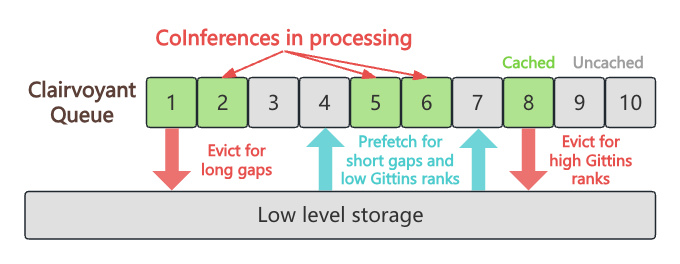
\includegraphics[width=1\linewidth]{figures/ClairvoyantQueue.png}
%     \caption{Illustration of resource eviction and prefetching between high and low-level storage using the Clairvoyant Queue.}
%     \label{fig:ClairvoyantQueue}
% \end{figure}





\subsubsection{Clairvoyant Queuing on Non-LLM Backends}
\label{subsubsec:queuing}
Serving LLM applications often requires diverse non-LLM bankends, the demands of which, as elaborated in \S\ref{subsec:demand_modeling}, are included in coinference modeling.
In production clusters concurrently serving massive LLM applications, it is possible that resource contention occurs on such non-LLM backends.
To elaborate, we focus on three typical types of LLM tools\footnote{
    While we pick up three relatively-simple tools for study in this part, we note that the general principle here can be applied to other professional tools, like the traditional symbolic solver used in AlphaGeometry~\cite{AlphaGeometry}.
}
(here we use a broad sense of \emph{tools} which refer to all the non-LLM components of LLM applications).
First, some code-writing applications~\cite{factool_code} may periodically verify the correctness of the generated code with a docker container (for better environment isolation); under insufficient CPU resources, the container launching requests would be queued on the scheduler. 
Second, LLM applications with RAG (like KBQAV~\cite{factool_kbqa}) may periodically search for documents from the websites, which, under limited network bandwidth, may cause non-negligible network queuing delay.
Third, LLM applications like HuggingGPT~\cite{hugginggpt} may call small models (hosted on dedicated GPU servers); facing bursting requests, such small models (constrained by the resources on the dedicated GPU servers) can also become a bottleneck. 

Note that our previous coinference scheduling priority is imposed to the LLM backends, and the above non-LLM tasks submitted to other backends are often handled by independent schedulers. % respectively managing each resource backend. 
For example, the docker launching requests would be submitted to a kubernetes scheduler.
Under the default strategy (e.g., FCFS) of those schedulers, it is possible that the non-LLM tasks of a high-priority application be queued for a long time, postponing the ultimate application completion.
To address this issue, we propose \emph{clairvoyant queuing on non-LLM backends}, which propagates the application priority to all the involved schedulers managing non-LLM backends.
This way, it can be ensured that both the LLM and non-LLM components of a high-priority application can be serviced without any queuing delay. 

% Non-LLM tasks also play a significant role in the inference processes of many applications. For instance, in certain code-writing applications~\cite{}, the system needs to verify the correctness of code generated by LLMs within a Docker container. Limited CPU resource makes a competition in creating containers. Additionally, in applications like KBQA~\cite{}, the system needs to search for information from websites, which, in environments with limited network resources, can lead to further competition. Moreover, applications such as HuggingGPT~\cite{} include DNN execution tasks that require GPU resources, creating yet another layer of competition. Resource contention causes these non-LLM tasks to wait for resources, potentially leading to higher-priority applications being blocked by lower-priority ones under the default FCFS scheduling strategy. To address this issue, we propagate the application’s priority to the non-LLM task execution manager, ensuring that tasks associated with higher-priority inferences are given precedence.


\subsubsection{Clairvoyant Backend Selection}
\label{subsubsec:selection}
So far, we focus on the cases with uniform LLM backends.
In practice, it is possible that the LLM service providers provision multiple backends each with distinct configurations~\cite{lin2024parrot}. % superiority.
For example, inference batch size is a critical hyperparameter that affects the latency-throughput trade-off: setting a larger batching size can yield a higher throughput (by 8.2$\times$) but the latency would also be higher (by $95\%$)~\cite{chen2023dissecting}.
For fast serving of LLM applications, we thus also need to properly select the backend for each stage based on its demand characteristics.

To address that problem, we can employ a heuristic, clairvoyant backend selection, which leverages our coinference demand information to judge backend suitability for each stage. 
Suppose there is a latency-sensitive backend (with batch size $B_\text{min}$) and a throughput-sensitive backend to choose---emulating a ``power-of-two-choices" scheduling space~\cite{sitaraman2001power}; given a stage, we schedule it to the latency-sensitive backend if its request parallelism is larger than $B\text{min}$, and otherwise to the throughput-sensitive backend, so as to attain fast stage completion. 
Our evaluations show that this heuristic can indeed work well in practice.
We note that the principle of clairvoyant backend selection can be extended to other multi-backend cases. 
For example, a cluster may have GPU nodes of different generations (with heterogeneous computation-memory ratios); based on the predicted request output length, we can schedule the (memory-intensive) long-output requests onto the backends with smaller computation-memory ratio (and vice versa), which can improve the overall resource utilization.


% In decoding processes characterized by low computation density, increasing the number of concurrent requests can significantly  improve resource utilization and overall throughput. However, this approach inevitably leads to increased latency for individual requests. Additionally, larger batch sizes require more GPU memory to store the KV Cache of active requests. To address this issue, service providers often deploy multiple backends with varied configurations to meet different SLOs. 
% Specifically, they configure backends with smaller batch sizes on GPUs with limited memory to cater to low-latency demands while saving costs, alongside backends with larger batch sizes to maximize throughput.

% Leveraging our coinference modeling, we can dynamically assess the number of concurrent requests within a coinference stage and intelligently route them to the most appropriate backend. For instance, in a map-reduce summarization application, map requests—which benefit from higher throughput—can be routed to backends with large batch sizes, thereby reducing stage latency. Conversely, single reduce requests, which require lower latency, will be directed to backends with smaller batch sizes, ensuring minimal request latency. This strategic routing optimizes the latency at each stage, thereby optimizing the latency of the entire application.

%%!TEX root = main.tex
\section{Implementation}
\label{sec:implementation}

\vspace{.3em}
\noindent\textbf{Coinference-Centric Serving System.} We implemented Hermes atop vLLM~\cite{kwon2023efficient}, an engine that supports advanced features for LLM serving, including paged memory management~\cite{kwon2023efficient} and continuous batching~\cite{yu_orca_2022}. Hermes comprises three main components: the Coinference Demand Model, Coinference Scheduler, and Coinference Resource Provisioning, totaling 4,100 lines of Python code. Additionally, we developed a comprehensive benchmark suite consisting of 11,300 lines of Python code, including 10 different application workloads.

\vspace{.3em}
\noindent\textbf{Coinference Demand Model.} 
We employ an \texttt{ApplicationPredictor} abstraction to model application-level information for coinferences, as shown in Fig.~\ref{fig:demand_model}. The \texttt{ApplicationPredictor} maintains a \texttt{Distribution} abstraction for each attribute of every stage, supporting the Gittins rank's cache update via \texttt{UpdateCache()} and query through \texttt{GetGittinsRank()}. Furthermore, the \texttt{ApplicationPredictor} also incorporates the \texttt{CorelationPredictor} described in \S\ref{subsec:demand_modeling}, using the pyAgrum~\cite{ducamp2020agrum} library for online predictions through \texttt{addEvidence()} and \texttt{makeInference()}.

\vspace{.3em}
\noindent\textbf{Coinference Scheduler.} 
We replaced vLLM's \texttt{scheduler} with the \texttt{CoInferenceScheduler} as a core component to support our coinference-centric serving while maintaining the original interface to accommodate the inference workflow. The \texttt{CoInferenceScheduler} organizes incoming requests into \texttt{CoInference}s comprising multiple \texttt{CoInferenceStages}. In each scheduling cycle, it triggers \texttt{update\_priority()} to refresh the priority of each \texttt{CoInference}. Subsequently, the \texttt{CoInferenceScheduler} build the \texttt{ClairvoyantQueue} with \texttt{ClairvoyantFilter} and pass the eviction and prefetching actions to the \texttt{BlockManager} and \texttt{LoRAManager}. Additionally, it also passes the priority to external tool managers via the OpenAI API.

\vspace{.3em}
\noindent\textbf{Coinference Resource Provisioning.} For KV cache, we extended the \texttt{BlockManager} to support a three-tier storage system, allocating and deallocating storage blocks on demand at the coinference level. We implemented layer-wise transmission of KV cache between host memory and HBM, and integrated this into popular LLMs such as LLaMA~\cite{touvron2023llama}, and OPT~\cite{zhang2022opt}\gz{a little strange? ontop vllm sounds better}, which are based on Transformers~\cite{wolf2019huggingface}. Additionally, we enabled multi-threaded eviction and prefetching of KV caches and LoRA adapters between disk and host memory. 
It is important to note that while Hermes supports storing KV caches on disk, read-back operations are only used for background thread prefetching. On-demand requests that attempt to read KV caches from the disk will instead directly reset to recompute, as the latency is measured more than two orders of magnitude greater in our test, and cannot be hidden even with layer-wise loading. To avoid excessive cache prefetching waste, we set the prefetch space to 60\% of the host memory. Given that the host memory size is $C$ and the average KV cache size of an application is $A$, the prefetch window length is $0.6 \cdot \frac{C}{A}$.
\chen{Add priority propagation and multi-end selection}
%!TEX root = main.tex
\section{Evaluation}
\label{sec:eval}


%\subsection{General Setups}
\begin{figure*}[t]
    \centering
    \begin{minipage}[t]{0.74\linewidth}
        \centering
        
\includegraphics[width=1\linewidth]{figures/evaluation_e2e.pdf}
            \vspace{-0.3in}

        \caption{
        % Average application completion times, dead-line satisfactory ratios, and time-per-token satisfactory ratios with various workload intensities in the End-to-end experiment.
        End-to-end LLM application performance of different schedulers against diverse service objectives (under different application arrival intensities).
        }
            \vspace{-0.1in}
        \label{fig:evaluation_e2e}
    \end{minipage}
    \hfill
    \begin{minipage}[t]{0.24\linewidth}
        \centering
        
\includegraphics[width=\linewidth]{figures/evaluation_sched.pdf}
            \vspace{-0.3in}

        \caption{Ablation study on the methods tackling demand dynamicity.} %Comparison between Hermes, its variants, and Hermes-Oracle.}
            \vspace{-0.1in}
        \label{fig:evaluation_sched}

    \end{minipage}
\end{figure*}

\phm{Implementations.}
We have implemented Hermes atop vLLM with over 4,100 lines of Python codes.
The functionalities of CoInference-aware Request Annotator in Fig.~\ref{fig:overview} are implemented in \texttt{CoinferenceAnnotator}, and we replaces the default vLLM scheduler to our \texttt{CoinferenceScheduler}.
Regarding intra-application resource provisioning, the \texttt{CoinferenceScheduler} passes the queue information to a series of lower-level resource managers---\texttt{BlockManager} and \texttt{LoRAManager} for cache management, \texttt{DockerManager}, \texttt{RetrievalManager} and \texttt{ModelManager} for non-LLM resource management, and \texttt{ServerSelector} for LLM backend selection. 
Additionally, we build a comprehensive benchmark suite consisting of 11,300 lines of Python code, which includes all of the ten application types depicted in Fig.~\ref{fig:app_structure}. 

\phm{Hardware Platform.}
We evaluate Hermes respectively with two different setups of single-GPU and multi-GPU experiments.
The large language models we use are LLaMA-7B and LLaMA-13B.
The single-GPU evaluations use a server with four 16-core AMD-EPYC-7302 CPUs, 128GB RAM, 4TB SSD and one NVIDIA A100-PCIE-40GB GPU. 
The multi-GPU evaluations use a server with four 20-core Intel-Xeon-Gold-6133 CPUs, 258GB RAM, 2TB SSD and four Tesla V100-PCIE-16GB GPUs. 
Both servers run CUDA 12.4.

% \phm{Hardware Platform.}
% We evaluate Hermes with the LLaMA-7B model respectively hosted on two backend servers: a single GPU server and a multi-GPU server. 
% The single-GPU server has four 16-core AMD-EPYC-7302 CPUs, 128GB DRAM, 4TB SSDs and one NVIDIA A100-PCIE-40GB GPU. 
% The multi-GPU server has four 20-core Intel-Xeon-Gold-6133 CPUs, 258GB DRAM, 2TB SSDs and four Tesla V100-PCIE-16GB GPUs. 
% Both servers run CUDA 12.4.

\phm{Workloads.}
For our experiments, we create a mixed workload suite with totally 500 LLM applications (each with distinct inputs from the original datasets). % from diverse categories.
In that workload suite, 20\% applications are multi-turn conversations requiring guaranteed TPT performance (TPT-sensitive), 20\% require meeting a preset deadline (DDL-sensitive), and the remaining 60\% target for short ACT (ACT-sensitive). 
To get the applications not involving TPT objectives, we randomly sample from the 9 non-conversation application families in Fig.~\ref{fig:app_structure}.
In particular, similar to prior work~\cite{qiao2021pollux, jayaram2023sia, zheng2023shockwave}, we set the sampling probability of small (EV, FEV, CC, ALFWI and KBQAV---usually less than 1 min), medium (CG and PE---usually between 1 and 10 min) and large (DM and MRS---usually longer than 10 min) applications to be 72\%, 26\%, and 2\%, respectively.
Meanwhile, for the TPT-sensitive applications, we set the TPT target as 0.1 s/token (given that typical human reading speed is less than 600 token per minute~\cite{reading_speed}).
For the DDL-sensitive applications, we set the deadlines by multiplying the original execution length by a random factor between 1.2 and 2, resembling some previous studies~\cite{narayanan2020heterogeneity, gu2023elasticflow}.
Regarding application submission, given a submission window of T, we let the submission interval follow a Poison distribution with the expectation be T/N (N is the total application number submitted in experiments). 

% \noindent\textbf{Workloads.}
% We developed a benchmark suite that includes the 10 workloads shown in Fig.~\ref{fig:app_structure}. 
% In our constructed end-to-end mixed workload, 20\% of the total submitted tasks in the trace are TPT-sensitive applications (specifically multi\_conversation), 20\% are DDL-sensitive applications, and 60\% are ACT-sensitive applications.
% Among non-TPT-sensitive applications, we categorized applications based on their execution time, and similar to prior work~\cite{qiao2021pollux, jayaram2023sia, zheng2023shockwave}, we set the probability of generating Small (0-1 min), Medium (1-10 min), and Large ($>$10 min) applications to be 72\%, 26\%, and 2\%, respectively.
% Small applications include Factool\_Generate-Code-Solution, Factool\_Knowledge-Based-QA, Factool\_Check-Math-Solution, ReAct\_Fact-Extraction-and-Verification, and ReAct\_ALFWorld; Medium applications include AutoGen\_CodeFeedback and HuggingGPT; and Large applications include LangChain\_MapReduce and GoT\_MergeDocuments. 
% The DDL values are determined by multiplying the original execution length by a random factor between 1.2 and 2, as done in previous studies~\cite{narayanan2020heterogeneity, gu2023elasticflow}.
% Following previous work~\cite{sheng2023s}, We generated application arrival times using a power-law distribution, with varying arrival rates represented by the exponent $\alpha$.


\subsection{End-to-end Scheduling Performance}




\phm{Setups.}
We first evaluate the scheduling performance of Hermes. 
We run an LLM inference engine on a single A100 GPU as the backend server, and submit all the 500 applications with the submission window respectively set to 10, 15 and 30 minutes (i.e., the workload intensity respectively be $3\times$, $2\times$ and $1\times$). 
%\noindent\textbf{Baselines.}
% We compare Hermes with three scheduling strategies: Request-FCFS, CoInference-FCFS, and Hermes-ACT, highlighting our approach to diverse application demands. 
% Request-FCFS schedules at the request level with an FCFS policy without awareness of higher-level applications, representing most existing LLM inference frameworks, such as vLLM~\cite{kwon2023efficient}. 
% CoInference-FCFS, on the other hand, is aware of higher-level applications and performs FCFS scheduling at the coinference level, exemplifying application-aware approaches like Parrot~\cite{lin2024parrot}. 
% Lastly, Hermes-ACT is an application-aware scheduler that optimizes for the best Application Completion Time (ACT) without considering other heterogeneous service objectives.
We compare Hermes with three scheduling strategies: Request-FCFS, Coinference-FCFS, and Hermes-ACT.
Request-FCFS schedules the request in the First-Come-First-Serve manner, which is the default scheduling policy in mainstream LLM serving frameworks like vLLM~\cite{vllm}.
Coinference-FCFS performs FCFS scheduling at the application level (as adopted in Parrot~\cite{lin2024parrot}), meaning that each request is scheduled based on the arrival time of the coinference it belongs to.
Hermes-ACT is a variant of Hermes which focuses only on minimizing average ACT. 
Regarding the metrics, for ACT-sensitive applications we measure the average ACT; for DDL-sensitive applications we measure the DDL Satisfactory Ratio, which is the proportion of DDL-sensitive applications that successfully meet their deadlines; for TPT-sensitive applications, we measure the TPT Satisfactory Ratio, which is the average proportion of checking points (once for every 10s) at which the TPT performance during the preceding interval (10s) satisfies the requirement.
%(each application has 30 time checking points that are evenly dispersed in its lifetime)\yfliu{How do we know the lifetime in runtime? Or we can set one checkpoint for each 5s, and any TPT violation in the interval between two adjacent checkpoints will set the TPT Satisfactory false. Then we calculate the TPT Satisfactory Ratio?}.

% \noindent\textbf{Metrics.}
% Hermes is designed to meet a wide range of application needs. Therefore, we primarily compare average application completion times, deadline satisfaction ratios, and time-per-token satisfaction ratios. The application completion time measures the duration from submission to completion for ACT-preferred applications. The deadline satisfaction ratio is defined as the proportion of DDL-sensitive applications that meet their deadlines. Similarly, the time-per-token satisfaction ratio reflects the percentage of TPT-sensitive applications that fulfill their TPT requirements.

\begin{figure}[t]
    \centering
    
\includegraphics[width=\linewidth]{figures/kvc_exp.pdf}
            \vspace{-0.3in}
    \caption{%(a) KV Cache Hit Ratio per Algorithm with different sizes of host memory, and (b) performance improvement on avg. ACT and makespan.
    Cache hit ratio (with different host memory sizes) and execution efficiency (measured with both average ACT and makespan) under Hermes, EPWQ and LRU.
    }
    \vspace{-0.1in}
    \label{fig:kvc_exp}
\end{figure}

\begin{figure}[t]
    \centering
    
\includegraphics[width=0.9\linewidth]{figures/evaluation_lora_load_miss_8rank.pdf}
            \vspace{-0.12in}
    \caption{Cumulative load delay and total miss count to load LoRA adapters from disk to memory.}
            \vspace{-0.1in}
    \label{fig:evaluation_lora}
\end{figure}

\begin{figure*}[t]
    \centering
            \vspace{-0.1in}
    
    \begin{minipage}[t]{0.707\linewidth}
        \centering
        
\includegraphics[width=1\linewidth]{figures/share_legend.pdf}
            \vspace{-0.3in}
        \caption{%Avg. ACT w/ or w/o resource provisioning for CPU, Network, and GPU resources with various workload intensities.
        Performance with and without clairvoyant queuing respectively on three different non-LLM backends in cases with resource contention.
        }
            \vspace{-0.1in}

        \label{fig:non-llm_resource_provisioning}
    \end{minipage}
    \hfill
    \begin{minipage}[t]{0.269\linewidth}
        \centering
        
\includegraphics[width=1\linewidth]{figures/dynamic_routing.pdf}
            \vspace{-0.3in}
        \caption{%Avg. ACT under different backend routing strategies with various workload intensities.
        Performance under different backend selection methods.
        }
            \vspace{-0.1in}

        \label{fig:multi-backend}
    \end{minipage}
\end{figure*}


% In the end-to-end experiments, we run an LLM inference engine (LLaMA 7B) on a single A100 GPU as the backend server, while a frontend benchmark suite simulates application arrivals. We use a mixed workload consisting of 500 application submissions and vary the submission window (with a baseline of 30 minutes, reduced by 1-3x) to evaluate the average application completion times, deadline satisfaction ratios, and time-per-token satisfaction ratios under different workload intensities. Fig.~\ref{fig:evaluation_e2e} presents the overall performance between Hermes and baseline strategies. 

\phm{Results.}
As shown in Fig.~\ref{fig:evaluation_e2e}, Hermes can perform much better than Request-FCFS and Coinference-FCFS in each case.
For example, when workload intensity is 1$\times$, the ACT performance of Hermes is 90.1\% (88.3\%) better than  Request-FCFS (Coinference-FCFS). 
% This demonstrate the effectiveness of our SRPT-style inter-scheduling schedulin
% We also note that in cases with intense contention, Request-FCFS performs in fact better than Coinference-FCFS, which is consistent with our toy example of Fig.
Meanwhile, by comparing the performance of Hermes and Hermes-ACT, we can learn that multi-objective compatibility is indeed quite necessary---especially in cases with intense contention: 
when the workload intensity is 3x, Hermes-ACT remarkably sacrifices the SLO performance in both DDL and TPT (by respectively 71.2\% and 93.6\% if compared with Hermes). 
Additionally, we also take notice of the scheduling overhead of Hermes, which remains below 1 ms in our measurements of each case, negligible compared to the time-consuming LLM computations. %, which is sufficient to provide a high throughput.
%This demonstrates the necessity to concurrently support diverse performance objectives in LLM application serving.
%\yfliu{In fact, for the Gittins policy scheduling part alone, our overheads in the evaluation test cases are all below 1 ms (even in the busiest trace, the submission rate does not exceed 2 app/s), which is sufficient to support high throughput.}
% \gz{5ms is not negligible when serving llama-7b on A100.}

% Regarding ACT performance, we observe that as the workload intensity increases from 1x to 3x, Hermes reduces the ACT by 90\% to 51\% compared to Request-FCFS and by 88\% to 57\% compared to CoInference-FCFS. 
% This is because a few large applications occupy a significant portion of the computational resources, and failing to be aware of and properly schedule these applications can result in severe head-of-line blocking.
% Under low workloads, Hermes achieves the same ACT as Hermes-ACT, while it improves by 2.9x, at 3x workloads. This is because Hermes not only optimizes ACT-sensitive applications but also prioritizes tasks with urgent SLO requirements. Sacrificing a portion of performance to enhance the satisfaction of SLO-sensitive applications is still an acceptable trade-off in terms of overall cluster user satisfaction.

% Regarding DDL performance, as the workload intensity increases from 1x to 3x, Hermes improves the DDL satisfaction ratio by 1.6x to 1.3x compared to Request-FCFS and by 4.5x to 3.7x compared to CoInference-FCFS. While Hermes-ACT achieves the same DDL performance to Hermes under low workload conditions, its DDL satisfaction ratio rapidly drops to only 29\% of that of Hermes as the load increases. This is because Hermes-ACT does not account for DDLs, optimizing the ACT for ACT-sensitive applications in the cluster at the expense of DDL-sensitive applications' performance.

% Regarding TPT performance, Hermes consistently maintains the highest TPT satisfaction ratio, as it treats TPT-sensitive applications with TPT violation risk as the highest priority. As the workload intensity increases from 1x to 3x, Hermes improves the TPT satisfaction ratio by 2.8x to 5.6x compared to Request-FCFS and by 2.4x to 1.9x compared to CoInference-FCFS. Hermes-ACT achieves similar TPT performance to Hermes under low load conditions. However, as the load increases, its TPT satisfaction ratio rapidly drops to just 6\% of that of Hermes, resulting in intolerable delays for multi-turn conversation users.

\subsection{$\!\!$Ablation Studies on Tackling Demand Dynamicity$\!\!$}

% \begin{figure}[t]
%     \centering
%     
\includegraphics[width=1\linewidth]{figures/evaluation_sched.pdf}
%     \caption{CDF of ACTs under Hermes, Hermes-Oracle, Hermes w/o Corelation Analysis, and Hermes w/o Gittins.}
%     \label{fig:evaluation_sched}
% \end{figure}

\phm{Setup.}
Recall that to handle demand dynamicity, we have adopted both correlation analysis (\S\ref{subsubsec:correlation_analysis}) and the Gittins policy (\S\ref{subsubsec:gittins}). 
To verify their effectiveness, we resort to a series of ablation experiments. 
We first disable the correlation analysis module and get \emph{Hermes-v1}.
Then we disable the Gittins policy (i.e., using the mean value of a distribution in SPRT scheduling), and further get \emph{Hermes-v2}. 
For reference, we also add an idealized baseline, Hermes-Oracle, which knows exactly the resource demand of each LLM application (by conducting a trial run with \texttt{temperature} set to 0).
%In our experiments, we submit 300 applications to the A100 server within a time window of 10 minutes, and measure the average ACT (normalized by that under standard Hermes).
In our experiments, we conduct two tests using LLaMA-7B and LLaMA-13B, respectively. 
LLaMA-7B uses two V100 GPUs with tensor parallel deployment, and LLaMA-13B uses four. 
We submit 300 applications to the V100 server within a time window of 10 minutes and measure the average ACT (normalized by that under standard Hermes).

\phm{Results.}
As shown in Fig.~\ref{fig:evaluation_sched}, without correlation analysis, the average ACT would be inflated by 15.3\% with the LLaMA-7B model. 
When the Gittins policy is further disabled, that performance degradation would increase to 47.5\%.
Such results confirm the indispensability of both the correlation analysis and the Gittins policy in tackling demand uncertainty.
Meanwhile, the performance gap between Hermes and Hermes-Oracle is less than 10\%, suggesting that Hermes can deliver near-optimal scheduling performance for LLM applications. %albeit confronting the dynamic demands of LLM applications.
We also notice that in each case, the performance of LLaMA-7B and LLaMA-13B are quite similar.
%\yfliu{Both LLaMA-7B and 13B behave similarly. In the case of LLaMA-13B, the average ACT would be inflated by 24.3\% without correlation analysis, and further increase to 54.2\% when the Gittins policy is disabled. }

% \noindent\textbf{Setup.}
% To evaluate the effectiveness of accurate conditional probability modeling and the Gittins index policy, we compare three variants of Hermes: Hermes w/o CA, where the corelation analysis is disabled; Hermes w/o Gittins, where Gittins index is replaced with mean-based remaining length prediction; and Hermes-Oracle, which has perfect knowledge of the application length upon submission. The experiments are conducted on an V100 GPU running an LLM inference engine (LLaMA 7B), using a workload of 300 application submissions within a 10-minute window.

% \noindent\textbf{Results.}
% According to Fig.~\ref{fig:evaluation_sched}, Hermes w/o CA increases ACT by 15\% compared to Hermes, while Hermes w/o Gittins increases ACT by 47\%. The correlation analysis provides Hermes with accurate distribution modeling, while the Gittins index policy guides Hermes in effectively utilizing this distribution—both are indispensable. The average ACT difference between Hermes and Hermes-Oracle is within 10\%, demonstrating that Hermes delivers near-optimal performance under scheduling uncertainties.


\subsection{Effectiveness of Clairvoyant Cache Management}



\phm{KV cache management.} 
To evaluate the effectiveness of Hermes in KV cache management, we submit 500 applications to the A100 server within 15 minutes.
We enable the KV cache to be evicted from GPU DRAM to CPU memory and also from the CPU memory to disk (whenever a layer is full), and loaded vice versa. 
In particular, we introduce two baselines: LRU and Evict/Prefetch-on-Waiting-Queue (EPWQ). 
EPWQ means to prioritize the KV cache based on the pending request queue (adopted in CachedAttention~\cite{gao2024cost}); yet, during the inter-stage gap of a coinference, since the downstream request is not in the queue, its desired KV cache would be of the lowest priority.
Under each method, we measure the total cache hit ratio (including both GPU and CPU cache hits) against different CPU memory sizes (8GB, 16GB and 32GB). 
As shown in Fig.~\ref{fig:kvc_exp}(a), Hermes consistently achieves the highest cache efficiency in each case, improving the overall cache hit ratio by up to $1.11\times$ ($0.33\times$) compared to LRU (EPWQ).
Fig.~\ref{fig:kvc_exp}(b) further depicts the average ACT and makespan under each scheme in the case with 32GB CPU memory.
It shows that Hermes can reduce the average ACT by 18\% (6\%) compared to LRU (EPWQ).

% \begin{figure}[h]
%     \centering
%     
\includegraphics[width=\linewidth]{figures/evaluation_kvc_jct_makespan.pdf}
%     \caption{The avg. JCT and makespan for each algorithm of KV cache provisioning.}
%     % \label{fig:bayes effect}
% \end{figure}

\phm{LoRA cache management.} 
% In terms of KV cache and LoRA, we conducted a comprehensive load testing on an A100 to validate the performance of Clairvoyant cache management. We compared Hermes with three representative cache management strategies: vLLM, LRU, and Evict/Prefetch on Waiting Queue (EPWQ). As one of the most popular LLM inference frameworks, vLLM only stores free prefix KV cache in the remaining GPU space and does not utilize memory and disk as temporary storage. In contrast, we expand storage to include memory and disk, managing it with LRU, which we denote as one of our baselines. EPWQ is an enhanced cache management strategy based on information from the upper scheduler, actively evicting and prefetching the corresponding KV cache and LoRA adapters based on the requests waiting in the queue, reflecting the caching management concepts from the latest works, S-LoRA~\cite{sheng2023s} and CacheAttention~\cite{gao2024cost}. 
To evaluate Hermes performance in LoRA caching, we compare Hermes with EPWQ, LRU, and No-Cache (i.e., not storing LoRA in host memory, which is also the default setting of vLLM). 
We set \texttt{max-loras} (the maximum number of parallel processes per iteration) to 10, \texttt{max-cpu-loras} (the number of LoRA caches that can be stored in CPU memory) to 20, and use totally 200 LoRA adapters for LLaMA 7B with a rank of 8. 
We submit a 25-minute workload containing 1,000 applications, with each application randomly assigned to one of the LoRA adapters (all requests of an application use the same LoRA).
Fig.~\ref{fig:evaluation_lora} shows the load latency and miss count under each scheme.
According to Fig.~\ref{fig:evaluation_lora}, compared to the second best (EPWQ), Hermes can reduce the LoRA load latency by 45\%, and reduce the number of LoRA misses by 55.2\%.

% \noindent\textbf{Results.}
% To evaluate the total cache hit ratio (including both GPU and CPU cache hits), we run a LLaMA 7B under different cache management strategies and varying sizes of host memory. As shown on the left side of Fig.~\ref{fig:kvc_exp}, we observe that Hermes consistently achieves the highest cache efficiency across all cache sizes. With 8 GB of host memory, Hermes improves the overall cache hit rate by 1.76x, 1.11x, and 0.33x compared to vLLM, LRU, and EPWQ, respectively. With 32 GB of host memory, Hermes achieves a 5.38x, 1.18x, and 0.33x improvement in the overall cache hit rate compared to vLLM, LRU, and EPWQ, respectively. The right side of Fig. 10 shows the performance improvement provided by Hermes with 32 GB of host memory: it reduces the average ACT by 20\%, 18\%, and 6\% compared to vLLM, LRU, and EPWQ, respectively.


% \subsection{Performance of LoRA Management}

% \noindent\textbf{Setup.}
% In the LoRA evaluation, we mainly compare Hermes with EPWQ, LRU, and No-Cache (i.e., not storing LoRA in host memory, which is also the default setting of vLLM). We set \texttt{max-loras} (the maximum number of parallel processes per iteration) to 10, \texttt{max-cpu-loras} (the number of LoRA caches that can be stored in CPU memory) to 20, and use a total of 200 LoRA adapters of LLaMA 7B with a rank of 8. We submit a 25-minute workload containing 1,000 applications, with each application randomly assigned to one of 200 LoRA adapters, and all requests for each application using the same LoRA.

% \noindent\textbf{Results.}
% From Fig.~\ref{fig:evaluation_lora}, we can see that Hermes reduces the number of LoRA cache misses by 55\%, 71\%, and 87\% compared to EPWQ, LRU, and No-Cache, respectively, and reduces the synchronous read time by 45\%, 65\%, and 84\%.

\subsection{$\!\!\!\!\!$Effect of Clairvoyant Queuing on Non-LLM Backends$\!\!\!\!\!\!\!\!$}

% \noindent\textbf{Resource Provisioning for Non-LLM task.}
% To assess the efficiency of non-LLM resource provisioning, we conducted three experiments focused on CPU, network, and GPU resources individually. We selected Code Feedback (AutoGen), KBQA (Factool), and HuggingGPT as workloads for these experiments, as each has distinct demands on these respective resources. We compared the average ACT scheduled by Hermes with and without resource provisioning under varying application arrival rates. The test environment consisted of a cluster with two V100 (16G) GPUs, and we hosted an LLM inference engine (LLaMA 7B) as the LLM backend. In the CPU resource experiment, we limited the total number of CPU cores to 40, with each Docker container allocated 2 cores. For the network, we restricted concurrent search requests to 4. In the GPU resource experiment, we limited concurrent requests to 15 based on the available GPU memory. The results, shown in ~Fig.\ref{fig:non-llm_resource_provisioning}, demonstrate that our resource provisioning mechanism can reduce the average ACT by up to 13\%. The improvement becomes more pronounced as the workload increases.

To assess the effectiveness of clairvoyant queuing on non-LLM backends (\S\ref{subsubsec:queuing}), we select three LLM applications, CG, KBQAV and PE, which respectively demands docker (to test code in a virtual environment), network (to search knowledge from the web) and GPU (to run the small models) resources.
The test environment contains two V100 (16G) GPUs serving the LlaMA-7B model.
% Yi-6B\yfliu{LLaMA-13B if four V100 GPUs}\gz{two V100 GPUs serving LlaMA-7B actually} model deployed in tensor parallel paradigm.
We build a prototype where each of the above resource backends is managed by an independent scheduler with limited service concurrency (for simplicity we manually set such limitation). 
For Docker backend, we limit the total number of CPU cores to 40, with each Docker container allocated 2 cores; for the network backend, we restrict the remote searching concurrency to 4; for the GPU backend (for small models), we limit the maximal concurrency to 15\%. % based on the available GPU memory.
In each case, we submit the selected applications under different arrival rates, 
%We vary the submission speed of each application, 
and Fig.\ref{fig:non-llm_resource_provisioning} depicts the average ACT.
%As shown in Fig.\ref{fig:non-llm_resource_provisioning}, 
Compared with the default case where each backend queues the request independently in FCFS order, Hermes can reduce the average ACT by up to 13\%.


% \begin{table}[htbp]
%     \centering
%     \begin{tabular}{cccc}
%     \hline
%     provision resource  & w/o Provision & w Provision \\
%     \hline
%     CPU & 232.9s & 209.8s \\
%     Network & 44.9s & 39.8s \\
%     GPU & 141.3s & 130.4s \\
%     \hline
%     \end{tabular}
%     \caption{Average ACT with or without Resource Provisioning}
%     \label{tab:tool_provisioning}
% \end{table}



\subsection{Effectiveness of Clairvoyant Backend Selection}
% In~Fig.\ref{fig:multi-backend}, we further evaluated the effectiveness of our multiple backends routing mechanism. We deployed two LLM engines (LLaMA 7B) in a cluster with four V100 (16G) GPUs, utilizing tensor parallelism with two GPUs per engine. The batch size for one backend was configured to 32 to achieve higher throughput, while the other backend had a batch size set to 8 for lower latency. We submitted map-reduce summarization applications as the primary workload and code generation applications (Factool) at varying rates as the background workload. We compared the average ACT when using our dynamic routing strategy against two other routing strategies that direct target applications to a single backend.

% When the background workload is light, routing applications directly to the backend with a large batch size achieves a low ACT. It can efficiently handle numerous map requests concurrently with a high throughput. Additionally, since only a few other requests are batched alongside the single reduce request, it does not significantly increase delay. In contrast, the backend with a small batch size struggles to manage the high volume of parallel requests during the map stage, leading to the worst performance. As the background workload increased, directly routing a single reduce request to the backend with a large batch size leads to longer completion times due to the batching with other requests. Thanks to our Coinference modeling, we can accurately perceive the parallelism of each stage. This enables a dynamic routing strategy that effectively assigns stages with low parallelism to the small backend and stages with high parallelism to the large backend. This approach consistently delivers optimal performance.

We further evaluate the effectiveness of our automatic backend selection method.
To that end, we deploy two LLaMA-7B backends with four V100 GPUs (each model deployed with two GPUs):
% two A100\yfliu{2 $*$ V100?}\gz{4 V100, in the platform part, we don't have 2 A100.} GPUs: 
the batch size for one backend is configured to 32 for high throughput, and the other to 8 for low latency.
The schemes compared are our clairvoyant backend selection strategy (i.e., try using throughput-first backend for stages with parallelism larger than 8, and try using the latency-first backend otherwise) and two naïve strategy that always choose a fixed backend (either 8 or 32).
We submit 500 LLM applications for multiple runs (in different runs we use different schemes but the application submission trajectory are fixed), and study the average ACT of those applications with non-trivial stage parallelisms (i.e., larger than 1). %\gz{result is strange in this way}
% the MapReduce Summarization applications (a typical application type containing stages with multiple requests).
Such experiments are repeated under different application arrival rates.
As shown in Fig.~\ref{fig:multi-backend}, in any case, our clairvoyant backend selection strategy can always make the best performance.




% \subsection{Overheads}

% \begin{figure}[t]
%     \centering
%     
\includegraphics[width=0.5 \linewidth]{figures/evaluation_overhead.pdf}
%     \caption{The median policy runtime for Hermes scheduler across different application arrive rates. The error bars indicate the 25$^{th}$ and 75$^{th}$ percentiles.}
%     \label{fig:overhead}
% \end{figure}

% To evaluate the complexity of Hermes, we measure its overhead across various application arrival rates. It is important to note that each application generates a series of requests, so the request arrival rate is often several times higher. As shown in Fig.~\ref{fig:overhead}, Hermes' computational overhead remains below 5 ms, which is sufficient to provide a high throughput.

%%!TEX root = main.tex
\section{Related Work}
\label{sec:related}
\chen{More optimization techniques to improve LLM inference}

In the literature, a bewildering array of research works have appeared on improving LLM inference performance \ys{avoid using fancy words.. make it simple. it looks like AI-generated text.}.
In \emph{operator implementation} aspect, the FlashAttention~\cite{dao2022flashattention} and FlashDecoding~\cite{hong2024flashdecoding} style algorithms are commonly adopted to realize efficient LLM inference by integrating IO awareness. 
In \emph{model deployment} aspect, model-quantization~\cite{frantar2022gptq,kim2023squeezellm}, paged-attention~\cite{kwon2023efficient} and prefill-decode-separation~\cite{zhong_distserve_2024,agrawal_taming_2024} methods have been proposed to maximize backend utilization.
In \emph{inference algorithm} aspect, continuous batching~\cite{yu_orca_2022} and speculative decoding methods~\cite{miao2023specinfer,cai2024medusa} are also applied to improve the inference throughput.
In \emph{request scheduling} aspect, a series of request-level scheduling algorithms like FastServe~\cite{wu2023fast} and Llumnix~\cite{sun2024llumnix} have emerged to improve the overall serving performance. 

\subsection{LLM Optimization Aware of Demand Dynamicity}
Some studies also notice the demand dynamicity on individual request level.  
In \emph{efficient inference} aspect, speculative decoding methods~\cite{miao2023specinfer,cai2024medusa} use a draft model to predict several subsequent tokens efficiently, enable the LLM to decode multiple tokens within the time frame if predictions are right. However, such works address demand dynamics within the constraints of a single request's upcoming outputs and carry the risk of increased overhead. the method of continuous batching~\cite{yu_orca_2022} has been proposed to mitigate uncertainties related to decoding length, allowing new requests to be added after the completion of an existing one. Although this work enhances efficiency, it does not address the underlying issues through prediction. 
In \emph{scheduling} aspect, Fastserve~\cite{wu2023fast} employs a multi-level feedback queue for priority management and predicts the remaining length of requests, enabling shorter requests to be executed first and avoiding head-of-line blocking. Nonetheless, this approach neglects their stage-level characteristics, and fails to consider the ACT. VTC~\cite{sheng2024fairness} introduces a novel cost function based on virtual token count to fairness. While this work takes into account the execution history of requests across different clients, it fails to consider the structural information of the requests, thus remaining at the request level.

Our approach not only considers the demand dynamicity at the request level but also accounts for parallelism and structural aspects, facilitating robust and accurate modeling and prediction for LLM applications.

\chen{how to handle demand dynamicity of LLM inferences}

\subsection{Response Length Prediction of LLM}

To get a higher LLM serving efficiency\gz{these stratrgise are not all designed to solve this problem. You can say e.g. to get a higher LLM serving efficiency ...}, many work have been done to predict the length of LLM output, which could be divided into two kinds of ideas: perceiving through LLM itself or predicting by other fine-tuned models. For works \emph{perceiving} through LLM itself, Perception in Advance (PiA)~\cite{zheng2024response} ask LLM to perceive output length before answering by add a question about output length in front of origin prompt. This method could achieve satisfying perception result, but may lead to undesirable consequences because it changes user's prompt. Perception Only (PO)~\cite{zheng2024response} decouples the prediction and generation processes but can't achieve performance as good as PiA. It could makes things worse that training the LLM specially to fix this problem is impossible. The works predicting by other fine-tuned models could use more flexible techniques. $S^3$~\cite{jin2023s} fine-tune a a Distilbert model to classify which length bucket the output sequence length falls into and could retrain it to learn from mistakes. TetriInfer~\cite{hu2024inference} also offline fine-tune a small LLM model to predict the generation length of LLM inference requests. ~\cite{fu2024efficient} apply Kendall’s Tau to measure the similarity between an LLM schedule and the oracle SJF/SRTF schedule, and show the strong correlation between Kendall’s Tau and  latency and throughput performance in practice. Then it uses ListMLE, a listwise ranking loss, to encouraging the model to predict a ranking close to the truth, other than predicting the length bucket of each request. 

Although these works have achieved promising results, they are limited to request level, with only limited information available for prediction. Our Hermes incorporates app-level structural information and contextual correlations, providing us with a richer set of information. This allows us to achieve better results with simpler methods.

\chen{Coflow Scheduling}
\subsection{Coflow Scheduling}
Coflow scheduling~\cite{chowdhury2012coflow} is a network scheduling technique which treats a group of related data flows, called a coflow, as a single unit for scheduling purposes. Often a communication stage cannot finish until all its flows have completed, so coflow process all these parallel flows with similar resource demand together to optimize the completion time of the entire group of flows (the coflow). Varys~\cite{chowdhury2014efficient}  proposes a inter-coflow scheduling policy for arbitrary coflows and focus on minimizing coflow’s completion time (CCT) and guaranteeing predictable completions within coflow deadlines. Unlike above jobs, Aalo~\cite{chowdhury2015efficient} requires no prior knowledge of coflow characteristics, making it simple for all data-parallel applications to use it. Although this notion is similar to coinference, coinference has more complex structure(e.g. branches and loops)
 and more uncertain demand quantity and involves more kinds of backend. So our work represents a fundamental innovation. Reducing dependence on prior knowledge, particularly in structure, is a key goal for our future efforts.
 
\chen{various job scheduling algorithms, SJF as a special case}

\subsection{Various Job Scheduling Algorithms}
There are various job scheduling algorithms for efficiently managing tasks and resources. First Come First Served (FCFS) is widely used in LLM scheduling because we can't know the response length of LLM inference. But it could cause Head-of-Line blocking, which is harmful to averge job completion time. Shortest Job First (SJF) or Shortest Remaining Job First (SRJF), let jobs with the shortest (remaining) execution time be executed first. SJF/SRJF is widely used in works with response length predictor to minimizes average waiting time, but may lead to "starvation" of longer jobs. Earliest Deadline First (EDF) schedule based on jobs' deadline. The job with the earliest deadline is executed first, optimizing deadline satisfaction. Multilevel Feedback Queue Scheduling, in which jobs can move between priority queues, could adapt to different workloads and dynamically prioritizes jobs. It could trade-off between different optimation objective.





%!TEX root = main.tex
    % \vspace{-0.2in}
\section{Conclusion}
\label{sec:conlucsion}

In this paper, we propose Hermes, an efficient serving system for LLM applications based on the coinference abstraction.
Hermes models a coinference as a list of stages, and depicts the dynamic resource demand in each aspect as a distribution.  
It further adopts the Gittins policy to optimize inter-coinference scheduling performance supporting diverse objectives.
For fast execution of each LLM application, Hermes adopts clairvoyant resource provisioning based on the profiled coinference demand on each backend.
Experimental results on popular workloads show that Hermes can remarkably improve the serving efficiency of LLM applications.

\bibliographystyle{plain}
\bibliography{main}
%% Bibliography
%\bibliography{bibfile}



\end{document}
